\section{Experimental Results}
\label{sec:experiment}

% \subsection{CPT Training and Transfer on Ascend NPUs}
% \label{subsec:cpt_training}


% % We evaluate the CPT pipeline from two perspectives. First, we assess whether
% % CPT training on Ascend NPUs is stable and produces meaningful domain adaptation
% % as measured by training dynamics, validation loss, and throughput. Second, we measure the downstream transfer
% % effect of CPT initialization on SFT through controlled CPT-to-SFT experiments
% % on four OR modeling benchmarks (Section~\ref{subsec:cpt_sft_transfer}).

% Following the evaluation protocol in Section~\ref{subsec:cpt_evaluation}, we evaluate CPT from two perspectives. First, we examine whether CPT on Ascend NPUs is stable in terms of loss trajectory, gradient norm, and learning-rate schedule. Second, we evaluate whether the resulting CPT checkpoint improves downstream SFT performance under matched SFT conditions.
% Figure~\ref{fig:cpt_training_dynamics} shows the training dynamics of the 500-iteration CPT run.

% % \begin{figure}[t]
% % \centering
% % \includegraphics[width=0.85\textwidth]{figures/cpt_plot.png}
% % \caption{Training dynamics of the run over 500 iterations. \textbf{(a) loss:} Language modeling loss (lm loss) and multi-token prediction loss (mtp loss). The LM loss decreases from 0.55 down to 0.30, while the MTP loss decreases rapidly from 1.0 to 0.40 and stabilizes after step 200. \textbf{(b) grad-norm:} The gradient norm steadily decreases from around 5.5 to 1.5, with a slight spike observed near step 470. \textbf{(c) learning-rate:} The learning rate schedule features a warmup phase reaching a peak of \(1 \times 10^{-6}\) at step ~50, followed by a cosine decay down to roughly \(1 \times 10^{-7}\).}
% % \label{fig:cpt_training_dynamics}
% % \end{figure}

% \begin{figure}[t] 
% \centering 
% \includegraphics[width=1\textwidth]{figures/cpt_plot.pdf} 
% \caption{CPT training dynamics over 500 iterations. \textbf{(a) Loss:} language modeling loss decreases from 0.55 to 0.30, while multi-token prediction loss drops from 1.0 to 0.40 and stabilizes after approximately 200 steps. \textbf{(b) Gradient norm:} the gradient norm decreases from around 5.5 to 1.5, with a mild spike near step 470. \textbf{(c) Learning rate:} the schedule uses a warmup phase peaking at \(1\times10^{-6}\) around step 50, followed by cosine decay to approximately \(1\times10^{-7}\).} \label{fig:cpt_training_dynamics} 
% \end{figure}

% The training curves indicate stable CPT optimization under the current Ascend configuration. Both LM loss and MTP loss decrease consistently, and the gradient norm remains controlled throughout most of the run. The isolated gradient spike near the end of training does not coincide with loss divergence, suggesting that the CPT pipeline is numerically stable in this setting.

% \paragraph{CPT-to-SFT Transfer.} We evaluate the downstream effect of CPT initialization using the matched CPT-to-SFT protocol defined in Section~\ref{subsec:cpt_evaluation}. Both the direct SFT route and the CPT-initialized SFT route use the same 10K chain-of-thought OR modeling samples, 220 SFT iterations, peak learning rate \(5\times10^{-6}\) with cosine decay, global batch size 128, and sequence length 8192. Therefore, performance differences between the two routes can be attributed to CPT initialization rather than different SFT data or optimization settings.

% % To evaluate whether CPT initialization benefits downstream SFT, we compare
% % two routes under identical SFT conditions:

% % \begin{align}
% % \text{Route A (direct SFT):}\quad&
% % \text{Base Model} \rightarrow \text{SFT}_{\text{10K CoT}} \\
% % \text{Route B (CPT $\rightarrow$ SFT):}\quad&
% % \text{Base Model} \rightarrow \text{CPT} \rightarrow \text{SFT}_{\text{10K CoT}}
% % \end{align}

% % The SFT stage uses 10K chain-of-thought OR modeling samples, 220 iterations,
% % peak learning rate $5\times10^{-6}$ with cosine decay, global batch size 128,
% % and sequence length 8192. All SFT hyperparameters are identical between the
% % two routes.

% %%%%%%%%%%%%%%%%%%

% % We evaluate on two complementary benchmarks:

% % \textbf{Bench4Opt Feasible}: Code-only feasibility evaluation.
% %     Measures whether the generated Gurobi program executes correctly and
% %     produces a feasible solution.
    
% % \textbf{Bench4Opt ORGEval}: Optimization modeling equivalence
% %     evaluation. Assesses whether the generated optimization model is
% %     structurally equivalent to the reference model, independent of
% %     implementation details.

% We report results on two Bench4Opt metrics. B4O-Feasible evaluates whether the generated Gurobi program executes successfully and produces a feasible solution. B4O ORGEval evaluates whether the generated optimization model is structurally equivalent to the reference model, independent of implementation details.


% \begin{table}[t]
% \centering
% \small
% \caption{CPT-to-SFT transfer results on Bench4Opt feasibility and ORGEval benchmarks.}
% \begin{tabular}{lcc}
% \toprule
% Model & B4O-Feasible & B4O ORGEval \\
% \midrule
% DeepSeek-V4-Flash~\citep{xu2026deepseek}-BF16
%     & 60.47\% & 34.26\% \\
% SFT$_{\text{10K CoT}}$
%     & 70.93\% & 48.73\% \\
% CPT $\rightarrow$ SFT$_{\text{10K CoT}}$
%     & \textbf{71.22\%} & \textbf{59.39\%} \\
% \bottomrule
% \end{tabular}

% \label{tab:cpt_sft_transfer}
% \end{table}

% % The transfer results show that CPT initialization provides positive gains on
% % both structured reasoning benchmarks:

% % \textbf{SFT alone is already a strong baseline.} Even without CPT, direct SFT
% % on the base model yields a 10.46pp improvement on B4O-Feasible (60.47\% $\to$
% % 70.93\%) and a 14.47pp improvement on B4O ORGEval (34.26\% $\to$ 48.73\%).
% % This indicates that the 10K chain-of-thought OR modeling samples themselves
% % contain rich domain signals, and SFT can effectively activate the model's
% % optimization modeling capabilities.

% % \textbf{CPT contributes most to deep structural reasoning.} On top of the SFT
% % baseline, CPT initialization further improves ORGEval by 10.66pp (48.73\%
% % $\to$ 59.39\%), while B4O-Feasible sees only a marginal gain of 0.29pp
% % (70.93\% $\to$ 71.22\%). ORGEval assesses structural equivalence between the
% % generated optimization model and the reference model---understanding
% % mathematical structure independent of surface-form expression---precisely the
% % kind of capability that domain-adaptive CPT is designed to inject. In contrast,
% % Feasible measures whether code runs and produces a feasible solution, a
% % capability largely covered by the SFT stage, leaving limited room for CPT
% % improvement.

% Table~\ref{tab:cpt_sft_transfer} shows that SFT alone is already a strong baseline. Compared with the base model, direct SFT improves B4O-Feasible from 60.47\% to 70.93\% and B4O ORGEval from 34.26\% to 48.73\%. This confirms that the 10K CoT OR modeling samples provide effective task-level supervision for activating optimization modeling capabilities.

% CPT initialization provides additional gains on top of this SFT baseline. The improvement is small on B4O-Feasible, increasing from 70.93\% to 71.22\%, but substantial on B4O ORGEval, increasing from 48.73\% to 59.39\%. This difference suggests that SFT is sufficient to improve executable feasibility in many cases, whereas CPT contributes more strongly to structural modeling competence. Since ORGEval emphasizes mathematical equivalence between the generated and reference optimization models, it is more directly aligned with the domain knowledge and modeling patterns introduced during CPT.

% % Overall,these results validate the core value proposition of
% % domain-adaptive CPT: targeted continued pre-training on OR-domain corpora can
% % further improve the most structurally demanding capabilities beyond what SFT
% % alone achieves. This provides a clear direction for future work in scaling up
% % CPT data volume and diversity.

% Overall, these results support the value of domain-adaptive CPT as a preparation stage for OR-oriented SFT. While direct SFT already improves task performance, CPT further strengthens the structurally demanding capabilities required for optimization model equivalence. This motivates scaling CPT with broader OR task coverage, higher-quality solver-verified documents, and retention-aware data mixtures in future experiments.

% % \subsection{SFT Training on Ascend NPUs}

% % Counter to the intuitive “more is better” scaling, increasing self‑distilled OR data from 3K to 50K did not monotonically improve performance—OptiBench even regressed at 50K, indicating that self‑distillation amplifies base‑model biases alongside correct patterns. We therefore shifted from quantity to quality: on the 10K base, we applied tiered cleaning (Clean‑only) and chain‑of‑thought enhancement (Clean‑cot).

% % \subsection{Stable SFT Training on Ascend 910C NPUs}
% % \label{subsec:sft}

% % Stable training is a prerequisite for meaningful downstream evaluation. If the training process is unstable, subsequent benchmark differences become difficult to interpret. In this project, we implement stable SFT training of DeepSeek-V4-Flash~\citep{xu2026deepseek} in a fully domestic environment with 8 nodes and 128 Ascend 910C NPUs in total.

% % Using the 50K self-distilled dataset as an example, we complete a relatively full-scale SFT verification run on DeepSeek-V4-Flash~\citep{xu2026deepseek}. The training configuration uses \texttt{GBS=128}, \texttt{MBS=1}, and \texttt{SEQ\_LEN=8192}. The model is trained for \texttt{800} steps, and checkpoints are saved at \texttt{200}, \texttt{400}, \texttt{600}, and \texttt{800} steps. The training log shows that the job successfully reaches \texttt{iteration 800/800}, without skipped iterations or NaN iterations. At the final iteration, the \texttt{lm loss} converges to approximately \texttt{0.079}, the \texttt{mtp\_1 loss} is approximately \texttt{0.093}, and the gradient norm remains within a normal range. The overall training curve decreases continuously and then gradually becomes stable.

% % As shown in Figure~\ref{fig}, these observations indicate that the current data preprocessing pipeline, MindSpeed-LLM training script, DeepSeek-V4-Flash~\citep{xu2026deepseek} base model, and 8-node 910C training environment form a reproducible and sustainable full-parameter SFT workflow. This provides a stable foundation for subsequent experiments on different data scales, data mixtures, and task-oriented data-distillation strategies.


% % \begin{figure}[t]
% %     \centering
% %     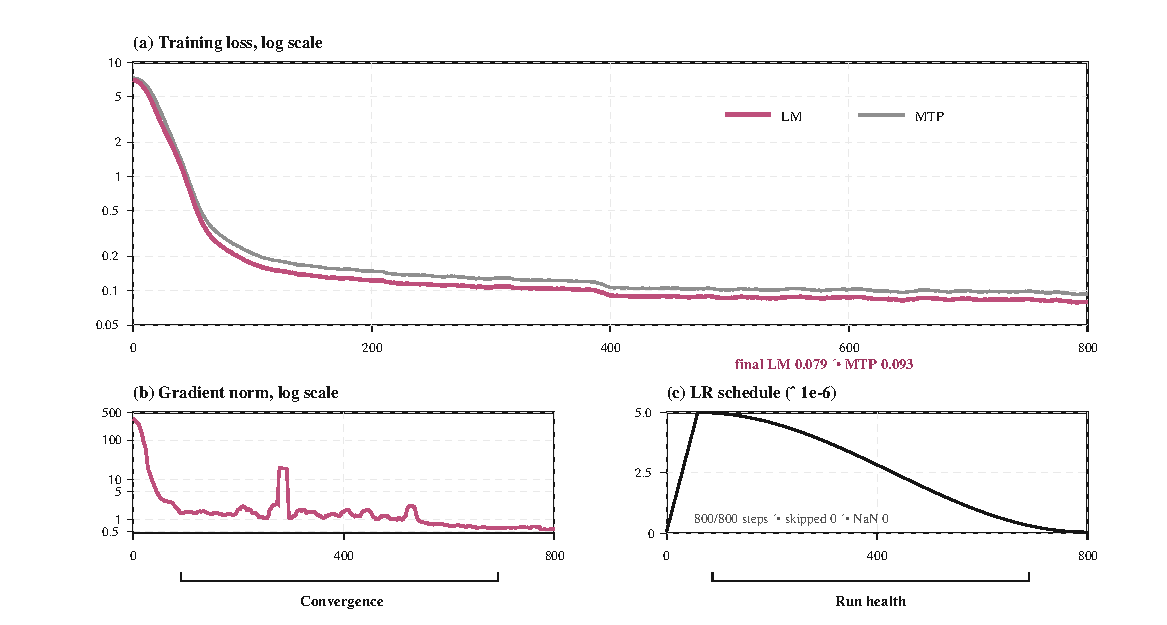
\includegraphics[width=\linewidth]{figures/fig_50k_sft_stability_paper.pdf}
% %     \caption{Training stability of the 50K self-distilled SFT run on Ascend 910C NPUs. The model is trained for 800 steps with \texttt{GBS=128}, \texttt{MBS=1}, and \texttt{SEQ\_LEN=8192}, and the training process reaches the final iteration without skipped or NaN iterations.}
% %     \label{fig:sft_50k_stability}
% % \end{figure}

% % The first systematic experiments on 3K, 10K, and 50K self-distilled data show that SFT brings two opposite effects. On the one hand, SFT clearly helps the model learn code-protocol tasks such as Bench4Opt. Taking DeepSeek-V4-Flash~\citep{xu2026deepseek}-B16 as the baseline, Bench4Opt feasible improves from 60.47 to 70.93 with SFT-10K, and Bench4Opt ORGEval improves from 34.26 to 47.21. These gains indicate that SFT makes the model more familiar with code-only output, \texttt{data.json} loading, Gurobi model construction, LP writing paths, and other benchmark-specific protocols.

% % On the other hand, SFT also weakens part of the model's original ability on natural-language modeling tasks. The baseline obtains 84.08 on NL4OPT, while SFT-10K obtains 81.66. Similarly, the baseline obtains 63.14 on OptiBench, while SFT-10K obtains 62.31. Further scaling to 50K does not solve this issue; instead, OptiBench decreases to 58.68. Since the 3K, 10K, and 50K settings follow almost the same construction design, the degradation of 50K is difficult to explain as a data-mixture change. A more plausible explanation is that continuous iterative distillation introduces lower-quality samples and amplifies the model's own noise.

% % \begin{table}[t]
% % \centering
% % \small
% % \begin{tabular}{lcccc}
% % \toprule
% % Model & NL4OPT & OptiBench & B4O-Feasible & B4O ORGEval \\
% % \midrule
% % DeepSeek-V4-Flash~\citep{xu2026deepseek}-B16 & 84.08 & 63.14 & 60.47 & 34.26 \\
% % SFT-3K  & 80.62 & 60.66 & 69.19 & 43.65 \\
% % SFT-10K & 81.66 & 62.31 & 70.93 & 47.21 \\
% % SFT-50K & 82.01 & 58.68 & 70.35 & 45.94 \\
% % \bottomrule
% % \end{tabular}
% % \caption{Systematic comparison of SFT data scales on OR modeling benchmarks.}
% % \label{tab:sft_scale_comparison}
% % \end{table}

% % Table~\ref{tab:sft_scale_comparison} leads to two conclusions. First, SFT is effective; otherwise, Bench4Opt would not show such substantial improvement. Second, SFT is not a monotonic scale-up game. If scale alone were sufficient, SFT-50K would not underperform SFT-10K, and the uncleaned SFT-10K would not fall below the baseline on NL4OPT and OptiBench. Failure analysis further explains this contradiction. Self-distillation can amplify the correct modeling habits of the base model, but it can also amplify the systematic weaknesses of the base model. Therefore, the problem of 50K is not simply that the dataset is too large, but that more weakly verified self-distilled samples assign a larger weight to noisy training signals. This is why the next step does not continue to scale the same pipeline to 100K, but instead returns to the 10K data for fine-grained cleaning.

% \subsection{SFT Stability, Scaling, and Cleaning Analysis}
% \label{subsec:sft_training_cleaning}

% Stable training is a prerequisite for meaningful downstream evaluation. If the training process is unstable, subsequent benchmark differences become difficult to interpret. In this project, we implement stable SFT training of DeepSeek-V4-Flash~\citep{xu2026deepseek} in a fully domestic environment with 8 nodes and 128 Ascend 910C NPUs in total.

% Using the 50K self-distilled dataset as an example, we complete a relatively full-scale SFT verification run on DeepSeek-V4-Flash~\citep{xu2026deepseek}. The training configuration uses \texttt{GBS=128}, \texttt{MBS=1}, and \texttt{SEQ\_LEN=8192}. The model is trained for \texttt{800} steps, and checkpoints are saved at \texttt{200}, \texttt{400}, \texttt{600}, and \texttt{800} steps. The training log shows that the job successfully reaches \texttt{iteration 800/800}, without skipped iterations or NaN iterations. At the final iteration, the \texttt{lm loss} converges to approximately \texttt{0.079}, the \texttt{mtp\_1 loss} is approximately \texttt{0.093}, and the gradient norm remains within a normal range. The overall training curve decreases continuously and then gradually becomes stable.

% As shown in Figure~\ref{fig:sft_50k_stability}, these observations indicate that the current data preprocessing pipeline, MindSpeed-LLM training script, DeepSeek-V4-Flash~\citep{xu2026deepseek} base model, and 8-node 910C training environment form a reproducible and sustainable full-parameter SFT workflow. This provides a stable foundation for subsequent experiments on different data scales, data mixtures, and task-oriented data-distillation strategies.

% \begin{figure}[t]
% \centering
% 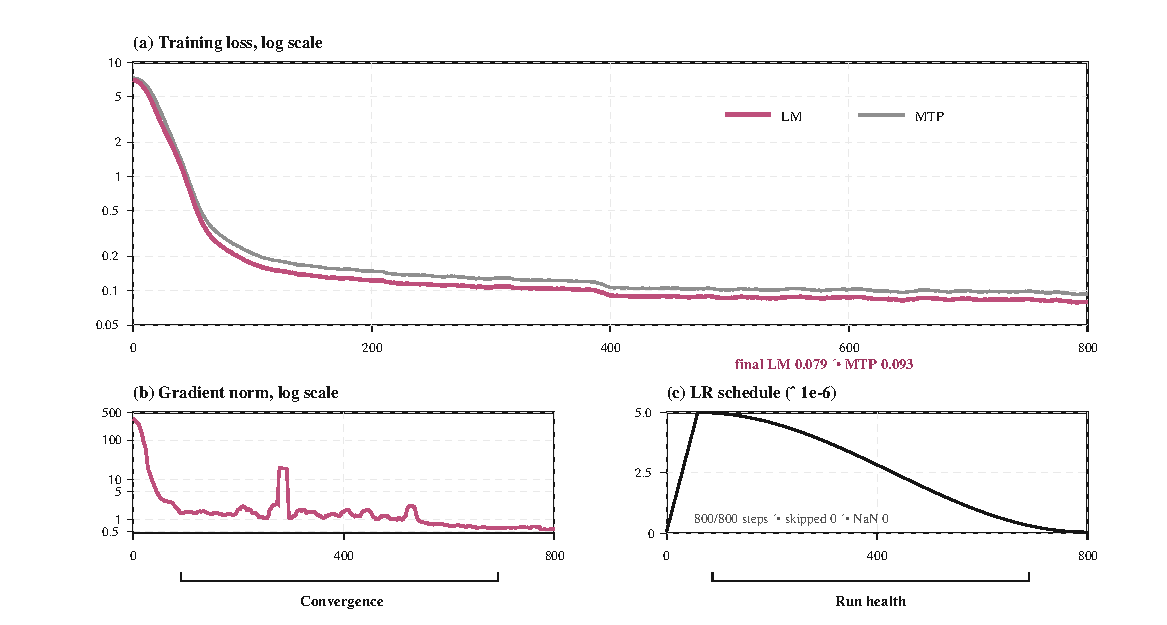
\includegraphics[width=\linewidth]{figures/fig_50k_sft_stability_paper.pdf}
% \caption{Training stability of the 50K self-distilled SFT run on Ascend 910C NPUs. The model is trained for 800 steps with \texttt{GBS=128}, \texttt{MBS=1}, and \texttt{SEQ\_LEN=8192}, and the training process reaches the final iteration without skipped or NaN iterations.}
% \label{fig:sft_50k_stability}
% \end{figure}

% The first systematic experiments on 3K, 10K, and 50K self-distilled data show that SFT brings two opposite effects. On the one hand, SFT clearly helps the model learn code-protocol tasks such as Bench4Opt. Taking DeepSeek-V4-Flash~\citep{xu2026deepseek}-B16 as the baseline, Bench4Opt feasible improves from 60.47 to 70.93 with SFT-10K, and Bench4Opt ORGEval improves from 34.26 to 47.21. These gains indicate that SFT makes the model more familiar with code-only output, \texttt{data.json} loading, Gurobi model construction, LP writing paths, and other benchmark-specific protocols.

% On the other hand, SFT also weakens part of the model's original ability on natural-language modeling tasks. The baseline obtains 84.08 on NL4OPT, while SFT-10K obtains 81.66. Similarly, the baseline obtains 63.14 on OptiBench, while SFT-10K obtains 62.31. Further scaling to 50K does not solve this issue; instead, OptiBench decreases to 58.68. Since the 3K, 10K, and 50K settings follow almost the same construction design, the degradation of 50K is difficult to explain as a data-mixture change. A more plausible explanation is that continuous iterative distillation introduces lower-quality samples and amplifies the model's own noise.

% \begin{table}[t]
% \centering
% \small
% \caption{Systematic comparison of SFT data scales on OR modeling benchmarks.}
% \begin{tabular}{lcccc}
% \toprule
% Model & NL4OPT & OptiBench & B4O-Feasible & B4O ORGEval \\
% \midrule
% DeepSeek-V4-Flash~\citep{xu2026deepseek}-B16 & 84.08 & 63.14 & 60.47 & 34.26 \\
% SFT-3K  & 80.62 & 60.66 & 69.19 & 43.65 \\
% SFT-10K & 81.66 & 62.31 & 70.93 & 47.21 \\
% SFT-50K & 82.01 & 58.68 & 70.35 & 45.94 \\
% \bottomrule
% \end{tabular}

% \label{tab:sft_scale}
% \end{table}

% Table~\ref{tab:sft_scale} leads to two conclusions. First, SFT is effective; otherwise, Bench4Opt would not show such substantial improvement. Second, SFT is not a monotonic scale-up game. If scale alone were sufficient, SFT-50K would not underperform SFT-10K, and the uncleaned SFT-10K would not fall below the baseline on NL4OPT and OptiBench. Failure analysis further explains this contradiction. Self-distillation can amplify the correct modeling habits of the base model, but it can also amplify the systematic weaknesses of the base model. Therefore, the problem of 50K is not simply that the dataset is too large, but that more weakly verified self-distilled samples assign a larger weight to noisy training signals. This is why the next step does not continue to scale the same pipeline to 100K, but instead returns to the 10K data for fine-grained cleaning.

% The SFT results after cleaning validate the effectiveness of the contract-aware cleaning and CoT enhancement framework introduced in Section~\ref{subsec:sft_cot_cleaning}. Compared with the uncleaned SFT-10K, clean-cot improves NL4OPT by 7.27 percentage points, OptiBench by 3.50 percentage points, and Bench4Opt ORGEval by 1.52 percentage points. This result suggests that the main issue of the 10K data is not insufficient scale, but semantic noise that is strong enough to damage natural-language modeling ability. Once such noise is systematically filtered and repaired, SFT no longer harms NL4OPT and OptiBench, but instead outperforms both the baseline and the original SFT-10K.

% \begin{table}[t]
% \centering
% \small
% \caption{Effect of data cleaning and chain-of-thought-oriented enhancement on OR modeling benchmarks.}
% \begin{tabular}{lcccc}
% \toprule
% Model & NL4OPT & OptiBench & B4O-Feasible & B4O ORGEval \\
% \midrule
% DeepSeek-V4-Flash~\citep{xu2026deepseek}-B16 & 84.08 & 63.33 & 60.47 & 34.26 \\
% SFT-10K & 81.66 & 62.67 & 70.93 & 47.21 \\
% Clean-only & 87.89 & 65.33 & \textbf{72.38} & 46.95 \\
% Clean-cot & \textbf{88.93} & \textbf{66.17} & 70.93 & \textbf{48.73} \\
% \bottomrule
% \end{tabular}

% \label{tab:sft_cleaning}
% \end{table}

% However, the gains of clean-cot are not uniformly distributed across all tasks. It is most effective on NL4OPT and OptiBench because these targets allow \texttt{<think>}, \texttt{<model>}, and \texttt{<python>} style answers. The structured modeling checklist can directly enter the training response and help the model learn explicit judgments about variable domains, objective direction, and constraint direction. By contrast, Bench4Opt feasible and ORGEval are code-only tasks, where explanatory chain-of-thought cannot appear in the output. Therefore, the advantage of clean-cot cannot be directly reflected in the response format. In the experiment, clean-only achieves 72.38 on Bench4Opt feasible, higher than the 70.93 of clean-cot. This suggests that for code-only tasks, excessive reliance on chain-of-thought enhancement does not necessarily bring additional benefits. These tasks require more specialized training on schema reading, index alignment, variable-family design, \texttt{model.write()} paths, and LP-structure consistency.

% Error analysis further reveals the boundary of cleaning-based enhancement. On NL4OPT, clean-cot reduces \texttt{wrong\_objective\_or\_model} errors from 52 cases before cleaning to 31 cases. On OptiBench, the same error type decreases from 154 to 128 cases, indicating that modeling checklists indeed reduce coarse errors at the objective and constraint levels. However, \texttt{nonlinear\_or\_bad\_gurobi\_form} errors on OptiBench do not decrease; instead, they increase from 49 to 56 cases. This shows that ordinary cleaning and short chain-of-thought enhancement can improve the question of what model should be built, but are insufficient to stably solve the question of how to correctly express nonlinear terms, ratios, averages, and quadratic terms in Gurobi. This observation motivates the subsequent design of nonlinear repair and specialized nonlinear/Gurobi synthetic data, rather than forcing all issues into a single clean-cot path.

% Therefore, the main conclusion of this SFT experiment is that chain-of-thought-oriented data enhancement is effective, but it must be constrained, contract-aware, and gated by reviewer and validation checks. Its value is not to make the model generate longer reasoning, but to inject the most error-prone optimization-modeling checkpoints into the training distribution in a stable form.

\label{subsec:stagewise_experimental_validation}

Our evaluation covers both halves of the full-stack effort in Section~\ref{sec:or_post_training_workflow}: the operator-level optimizations that raise device efficiency, and the post-training pipeline that turns the stabilized stack into downstream capability. We begin at the operator level and validate the two kernel-optimization strategies against the same DeepSeek-V4-Pro training workload whose bottlenecks motivated them (Section~\ref{sec:kernel_bottleneck}). Section~\ref{subsec:eval_aurakernel} evaluates AuraKernel on the heavy head of architecture-intrinsic kernels, where profiling-in-the-loop tuning reduces the per-invocation duration of the dominant sparse-attention and normalization kernels. Section~\ref{subsec:eval_operator_chain_fusion} evaluates the proactive operator-chain fusion on the fragmented, memory-bound tail, where collapsing framework-emitted eager chains into fused AscendC kernels removes redundant launches, intermediate tensors, and global-memory traffic. Because both are measured on the profiled training workload rather than on isolated microbenchmarks, the reported speedups attach directly to the device-time regimes identified in Section~\ref{sec:bottleneck}.

We then evaluate the post-training pipeline on Ascend 910C using
DeepSeek-V4-Flash as the experimental platform. We organize the experiments from infrastructure optimization to OR-specific model adaptation. We first verify that the training stack is stable on Ascend NPUs, retaining only the larger SFT stability run as the representative systems evidence. We then analyze the SFT scale and cleaning experiments, followed by the matched CPT$\rightarrow$SFT
transfer experiment. 
The final end-to-end result section is left as the summary comparison across Base, CPT, SFT, and CPT+SFT.


For clarity, the SFT labels in this section refer to two related but distinct points in the training trajectory. SFT-10K is the uncleaned 10K run used for scale analysis (Table~\ref{tab:sft_scale}) and as the pre-cleaning baseline in Table~\ref{tab:sft_cleaning}. Clean-CoT is the cleaned, CoT-enhanced checkpoint; the SFT row in the transfer and end-to-end tables (Tables~\ref{tab:cpt_sft_transfer} and~\ref{tab:main_results}) uses this matched-condition cleaned SFT checkpoint, so its 0-shot Pass@1 values align with the Clean-CoT row.

\subsection{Efficient Kernels via AuraKernel}
\label{subsec:eval_aurakernel}

\paragraph{Optimization targets.}
AuraKernel is applied along the two axes identified in Section~\ref{sec:kernel_bottleneck}: the dominant architecture-intrinsic kernels and the reduction-heavy framework operators that dominate the long tail. Table~\ref{tab:kernel_results} reports representative speedups on both axes, while Figure~\ref{fig:sparse_series} and Figure~\ref{fig:lightning_series} visualize the task-duration and pipeline-metric changes for sparse attention and the lightning indexer, respectively. To keep the numbers hardware-agnostic, we describe the gains through speedups and pipeline ratios rather than absolute latencies and analyze each axis in turn below.
\begin{table}[h]
\centering
\caption{Representative operators optimized by AuraKernel on Ascend 910C, reported as single-operator task duration. The sparse-attention forward and backward and the sparse lightning-indexer gradient are per-invocation durations measured in the end-to-end training context at two compression ratios (for the indexer, cmp.\ ratio $0$ is the full CFA path with RoPE and softmax, cmp.\ ratio $4$ is the SCFA path); the RMS-normalization kernels are measured at the operator level ($tp{=}2$, input $[B{\cdot}S{=}8192,\,H{=}64,\,D{=}512]$, BF16). Speedup is baseline/optimized.}
\label{tab:kernel_results}
\resizebox{\textwidth}{!}{%
\begin{tabular}{llccc}
\toprule
Operator & Context & Baseline (ms) & Optimized (ms) & Speedup \\
\midrule
\texttt{SparseAttnSharedkv}             & cmp.\ ratio $128$ & $0.88$ & $0.72$  & $1.23\times$ \\
\texttt{SparseAttnSharedkv}             & cmp.\ ratio $4$   & $4.17$ & $3.83$  & $1.09\times$ \\
\texttt{SparseAttnSharedkvGrad}         & cmp.\ ratio $128$ & $32.9$ & $26.5$  & $1.24\times$ \\
\texttt{SparseAttnSharedkvGrad}         & cmp.\ ratio $4$   & $24.3$ & $20.1$  & $1.21\times$ \\
\texttt{SparseLightningIndexerGradKLLoss} & cmp.\ ratio $0$ (CFA)  & $20.7$ & $17.9$ & $1.16\times$ \\
\texttt{SparseLightningIndexerGradKLLoss} & cmp.\ ratio $4$ (SCFA) & $7.22$ & $5.97$ & $1.21\times$ \\
\texttt{RMSNormWithoutWeightFwd}        & operator, $tp{=}2$ & $20.9$ & $1.76$  & $11.90\times$ \\
\texttt{RMSNormWithoutWeightBwd}        & operator, $tp{=}2$ & $27.7$ & $8.09$  & $3.42\times$ \\
\bottomrule
\end{tabular}
}
\end{table}

\begin{figure}[h]
\centering
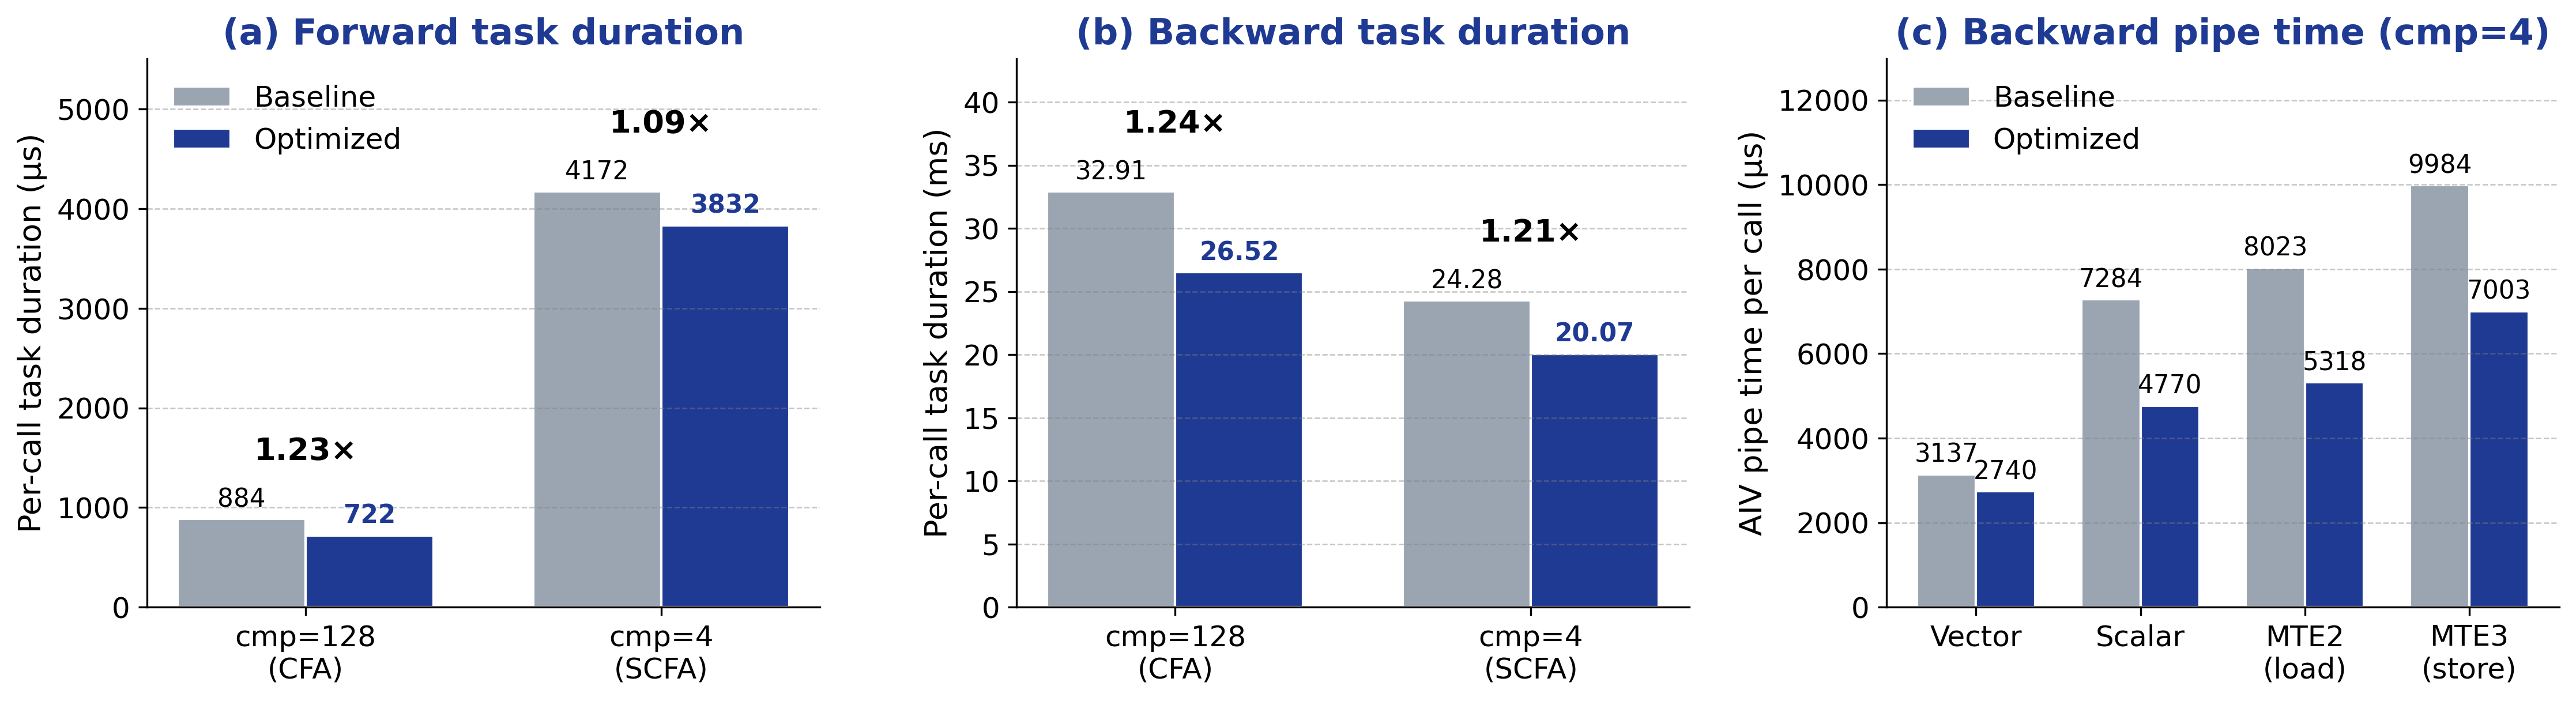
\includegraphics[width=\textwidth]{figures/sparse_series.png}
\caption{AuraKernel optimization of the shared-key-value sparse-attention kernels on Ascend 910C. (a)~Per-call forward task duration ($1.23\times$ at compression ratio $128$, $1.09\times$ at compression ratio $4$). (b)~Per-call backward task duration of \texttt{SparseAttnSharedkvGrad} ($1.24\times$ and $1.21\times$). (c)~AIV pipeline-time decomposition of the backward kernel at compression ratio $4$: the reductions concentrate in the memory-movement pipes (MTE2 load and MTE3 store) rather than in vector compute, confirming that the gain comes from cutting global-memory traffic.}
\label{fig:sparse_series}
\end{figure}

\begin{figure}[h]
\centering
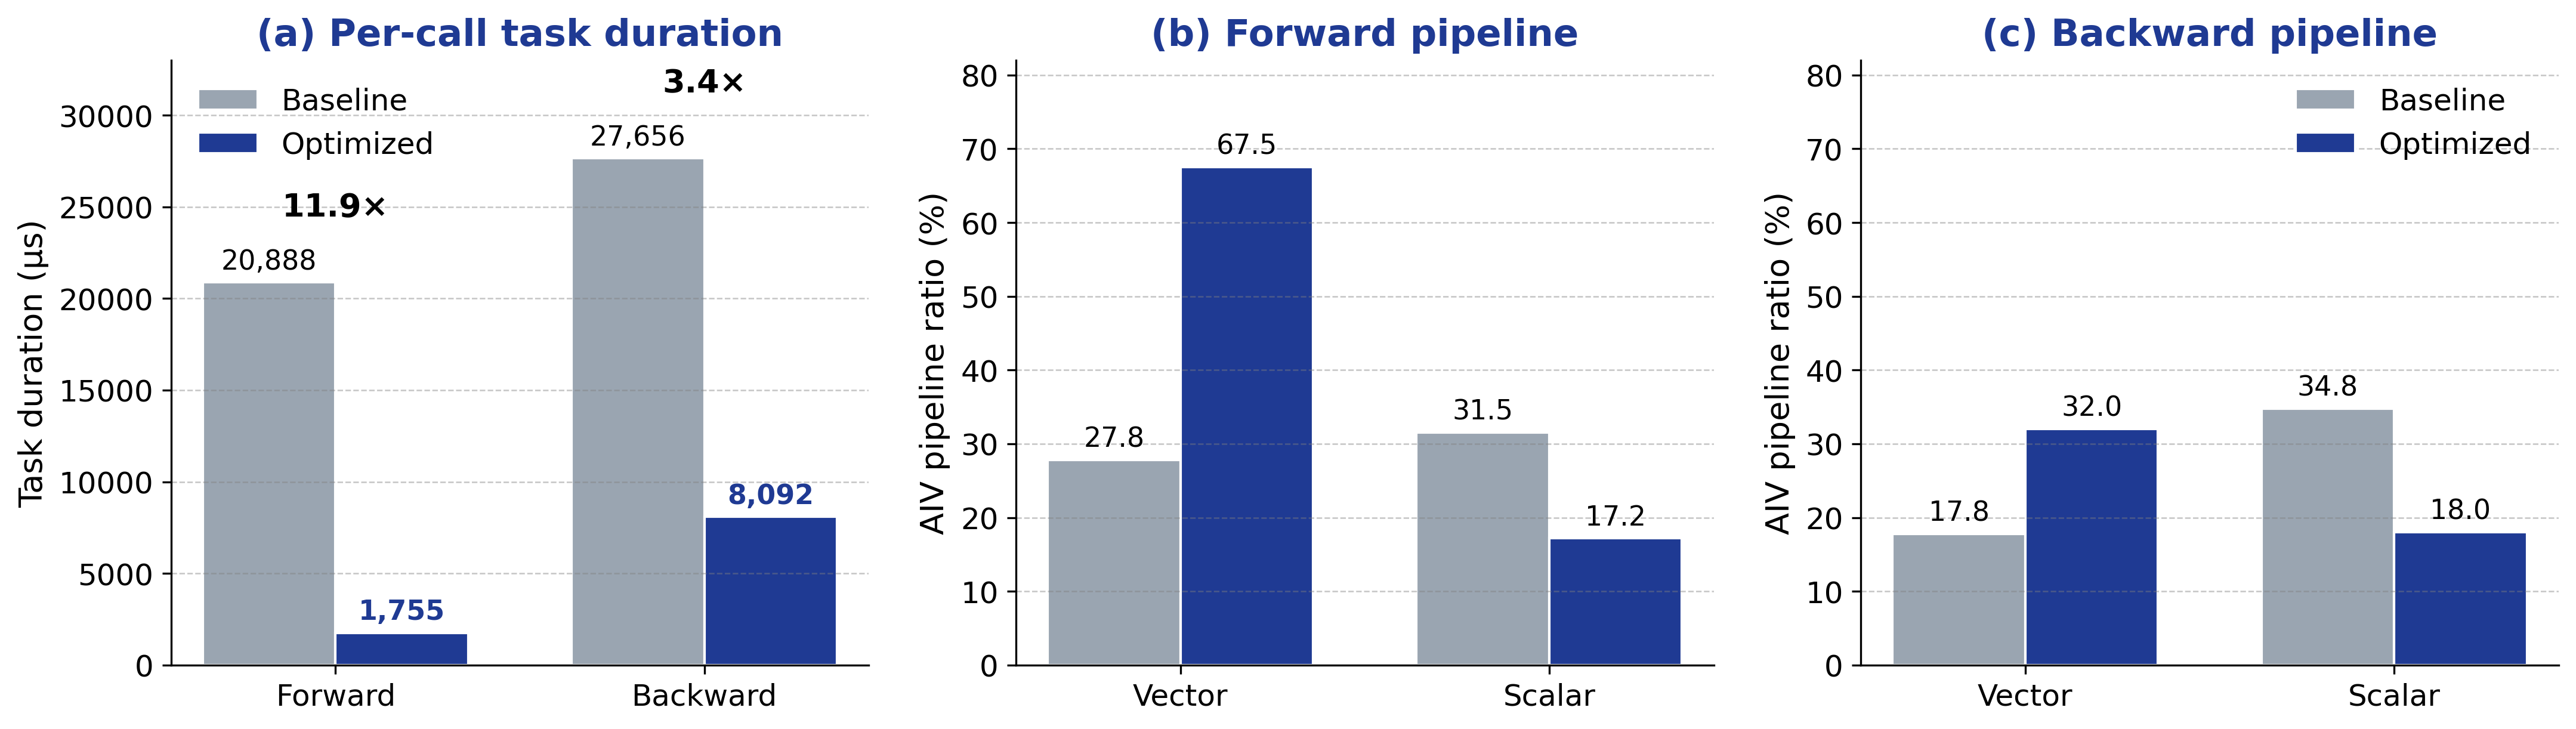
\includegraphics[width=\textwidth]{figures/rms_series.png}
\caption{AuraKernel optimization of the weight-free RMS-normalization kernels ($tp{=}2$). (a)~Per-call task duration speedup: forward $11.9\times$ and backward $3.4\times$. (b,c)~Duration-weighted AIV pipeline ratios before and after optimization: the vector-compute ratio rises (forward $27.8\%\rightarrow67.5\%$, backward $17.8\%\rightarrow32.0\%$) while the scalar ratio falls (forward $31.5\%\rightarrow17.2\%$, backward $34.8\%\rightarrow18.0\%$), showing that 2D head blocking, multi-row processing, and explicit FP32 accumulation turn a scalar/address-bound reduction loop into a vector-compute-dominated kernel.}
\label{fig:rms_series}
\end{figure}

\begin{figure}[h]
\centering
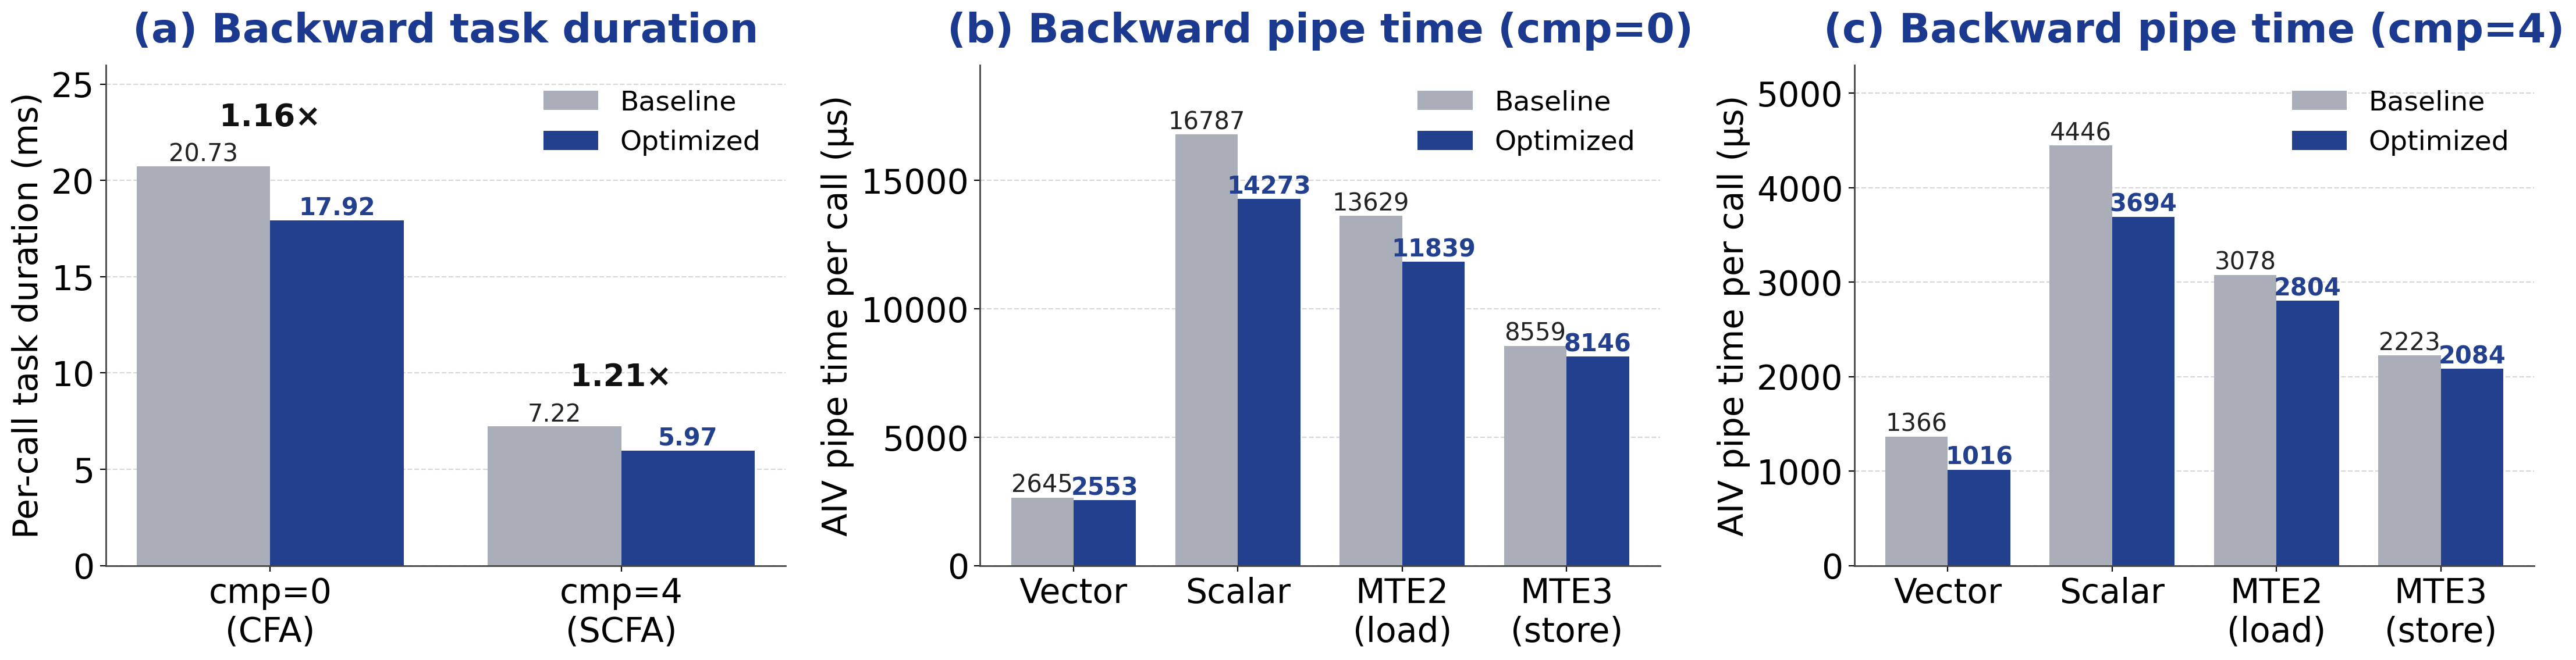
\includegraphics[width=\textwidth]{figures/lightning_series.png}
\caption{AuraKernel optimization of the sparse lightning-indexer gradient on Ascend 910C. (a)~Per-call backward task duration speedup, $1.16\times$ on the full CFA path (cmp.\ ratio $0$) and $1.21\times$ on the SCFA path (cmp.\ ratio $4$). (b,c)~AIV pipeline-time decomposition before and after optimization at the two ratios: the kernel is scalar- and load-bound, and the reductions concentrate in the scalar and MTE2-load pipes rather than in vector compute, consistent with cutting address-computation and global-memory-load traffic.}
\label{fig:lightning_series}
\end{figure}

\paragraph{Top hot-spot operators.}
The heavy head is formed by the architecture-intrinsic kernels of the DeepSeek-V4 hierarchical sparse attention, which Section~\ref{sec:kernel_bottleneck} identified as the largest single consumers of device time, with the shared-key-value sparse-attention backward alone at $\approx 16.33\%$ of per-step compute. Their metric-vector fingerprint is not compute-bound but movement- and scalar-bound: for \texttt{SparseAttnSharedkvGrad} the AIV load/store ratios (MTE2$+$MTE3) reach $\approx 0.559$ against a MAC ratio of only $\approx 0.10$, and the sparse lightning-indexer gradient is scalar- and load-bound (AIV scalar $\approx 0.81$, MTE2 load $\approx 0.66$ on the CFA path), so the duration floor is set by global-memory (GM) traffic and address computation rather than arithmetic. A top-$k$ locality analysis on real routing indices explains where this traffic originates: adjacent queries select almost identical compressed key-value blocks (adjacent-query Jaccard $\approx 0.998$ at $K{=}1024$), yet the baseline processes one query per task and re-gathers and re-scatters the same shared blocks once per query. AuraKernel maps this to two hardware-grounded rewrites: (i)~it batches consecutive queries per task and accesses the compressed side densely over the causal range instead of per-query sparse gather, cutting compressed-side GM traffic by roughly the batch factor; and (ii)~once batching shifts the floor onto the cube engine, it stores the heaviest FP32 cube$\rightarrow$vector hand-offs in BF16 to narrow the remaining GM round-trips, under an exact top-$k$ membership mask and gradient-magnitude and loss-stability gates that keep the rewrite numerically faithful. The gain lands on the modeled bottleneck: the sparse-attention backward improves by $1.24\times$ and $1.21\times$ at compression ratios $128$ and $4$, its forward by $1.23\times$ and $1.09\times$, and the lightning-indexer gradient by $1.16\times$ on the CFA path and $1.21\times$ on the SCFA path (Table~\ref{tab:kernel_results}, Figures~\ref{fig:sparse_series} and~\ref{fig:lightning_series}); in every case the per-call reduction concentrates in the MTE2/MTE3 load-store pipes, and additionally the scalar pipe for the indexer, rather than in vector compute, confirming that the improvement comes from removing GM traffic and address overhead rather than from raising raw compute utilization.

\paragraph{Triton-optimized operators.}
The long tail is carried by reduction-heavy framework operators expressed as Triton-Ascend kernels, which Section~\ref{sec:kernel_bottleneck} flagged as launch-fragmented and memory- and scalar-bound rather than compute-bound. Profiling localizes the cause to structural inefficiency inside these kernels: the weight-free RMS-normalization forward runs a serial per-head loop that leaves the vector engine idle behind a high scalar ratio, its backward emits poor scalar code because the reductions are not explicitly promoted to FP32, and several MHC operators accumulate through atomic-add or precede the main kernel with a standalone zero-init launch. Because these are Triton operators, AuraKernel restructures them within the Triton programming model, adjusting only host-side tiling and pipeline parameters while preserving the kernel mathematics: 2D head blocking and multi-row processing to replace the serial head loop, explicit FP32 accumulation and head-dimension unrolling, three-phase load-compute-store software pipelining to overlap the MTE2, vector, and MTE3 pipes, and elimination of atomic-add and standalone zero-init launches. A single campaign drives all $14$ Triton-Ascend operators (the RMS-normalization pair and the DeepSeek-V4 MHC family) to $100\%$ completion at a $2.06\times$ average and an $11.90\times$ best speedup, the backward RMS-normalization improving by $3.42\times$ (Table~\ref{tab:kernel_results}, Figure~\ref{fig:rms_series}). The gain shows up as a pipeline shift: the AIV vector-compute ratio rises sharply while the scalar ratio falls (RMS-normalization forward $27.8\%\rightarrow67.5\%$ vector and $31.5\%\rightarrow17.2\%$ scalar; backward $17.8\%\rightarrow32.0\%$ vector and $34.8\%\rightarrow\approx18\%$ scalar), turning scalar- and address-bound reduction loops into vector-compute-dominated kernels. The largest wins concentrate on reduction-class operators with structural inefficiency, whereas operators already at the bandwidth limit gain only a few percent.

\subsection{Performance Improvements from Kernel Fusion}
\label{subsec:eval_operator_chain_fusion}


\begin{table}[!ht]
\centering
\small
\caption{Operator-chain fusion results from the pre-optimization (fusion off) and post-optimization (fusion on) profiling traces, measured at global batch size $1024$. Operator counts are trace records attributed to the target module. ``Records'' gives the module-level count before and after fusion and its net change $\Delta$. ``Fused calls'' is the count of the inserted AscendC kernel, cross-checked against the post-optimization trace by matching operator name and type. ``Module time'' is the summed device task duration of the module before and after fusion, under the same submodule attribution. ``Per call'' divides each module time by the number of semantic invocations, so it reports how heavy one invocation of the eager chain is against its fused replacement. The speedup is identical whether read at the module or per-call level, because both share the same invocation count.}
\label{tab:operator_chain_fusion_results}
\resizebox{\textwidth}{!}{%
\begin{tabular}{@{}lccccc@{}}
\toprule
Optimization target & Fused kernel & \makecell{Records\\($\Delta$)} & \makecell{Fused\\calls} & \makecell{Module time\\(before\,$\rightarrow$\,after)} & \makecell{Per call\\($\mu$s)} \\
\midrule
mHC pre-projection &
\texttt{WindHcPreBmmForward} &
\makecell{$14336\rightarrow8064$\\$(-6272)$} &
$896$ &
\makecell{$1.287\rightarrow0.425$\,s\\$3.03\times$} &
\makecell{$1437\rightarrow474$} \\
mHC pre-projection backward &
\texttt{WindHcPreBmmBackward} &
\makecell{$21504\rightarrow17920$\\$(-3584)$} &
$448$ &
\makecell{$1.913\rightarrow1.019$\,s\\$1.88\times$} &
\makecell{$4270\rightarrow2274$} \\
mHC post-projection &
\texttt{WindMhcPostPart} &
\makecell{$7168\rightarrow3584$\\$(-3584)$} &
$896$ &
\makecell{$1.710\rightarrow0.624$\,s\\$2.74\times$} &
\makecell{$1908\rightarrow697$} \\
Limited SwiGLU forward &
\texttt{SwiGluLimitV2} &
\makecell{$5376\rightarrow896$\\$(-4480)$} &
$896$ &
\makecell{$1.480\rightarrow0.167$\,s\\$8.86\times$} &
\makecell{$1652\rightarrow186$} \\
Limited SwiGLU backward &
\texttt{SwiGluLimitBackwardV2} &
\makecell{$5824\rightarrow448$\\$(-5376)$} &
$448$ &
\makecell{$0.805\rightarrow0.246$\,s\\$3.27\times$} &
\makecell{$1797\rightarrow549$} \\
RoPE forward sites &
\texttt{WindScaleRope} &
\makecell{$14208\rightarrow2176$\\$(-12032)$} &
$2176$ &
\makecell{$1.421\rightarrow0.611$\,s\\$2.33\times$} &
\makecell{$653\rightarrow281$} \\
RoPE backward sites &
\texttt{WindScaleRopeGrad} &
\makecell{$15744\rightarrow2176$\\$(-13568)$} &
$1088$ &
\makecell{$1.599\rightarrow0.451$\,s\\$3.54\times$} &
\makecell{$1470\rightarrow415$} \\
\bottomrule
\end{tabular}}
\end{table}

We next evaluate the operator fusion and rewrite path in Section~\ref{sec:kernel_fusion}. The measurement unit is different from the AuraKernel results above. Whereas AuraKernel improves kernels that already appear as large execution units in the trace, this path changes the unit of execution itself. The baseline is therefore the complete eager chain emitted by Python, torch, and autograd for a model-level operation, or the generic Triton kernel that a stage was previously lowered into, not a single primitive operator selected from that chain. This distinction is important for interpreting the result: a fused or rewritten implementation may preserve the same mathematical work while removing the launches, intermediate tensors, dtype round trips, and scatter-style writebacks that surrounded it in the original trace, and while relocating the remaining arithmetic onto a substrate with explicit on-chip residency and pipeline scheduling. We present the targets in the order of Section~\ref{sec:kernel_fusion}: the mHC suite first, then limited SwiGLU and unified RoPE.


\begin{figure}[htbp]
\centering
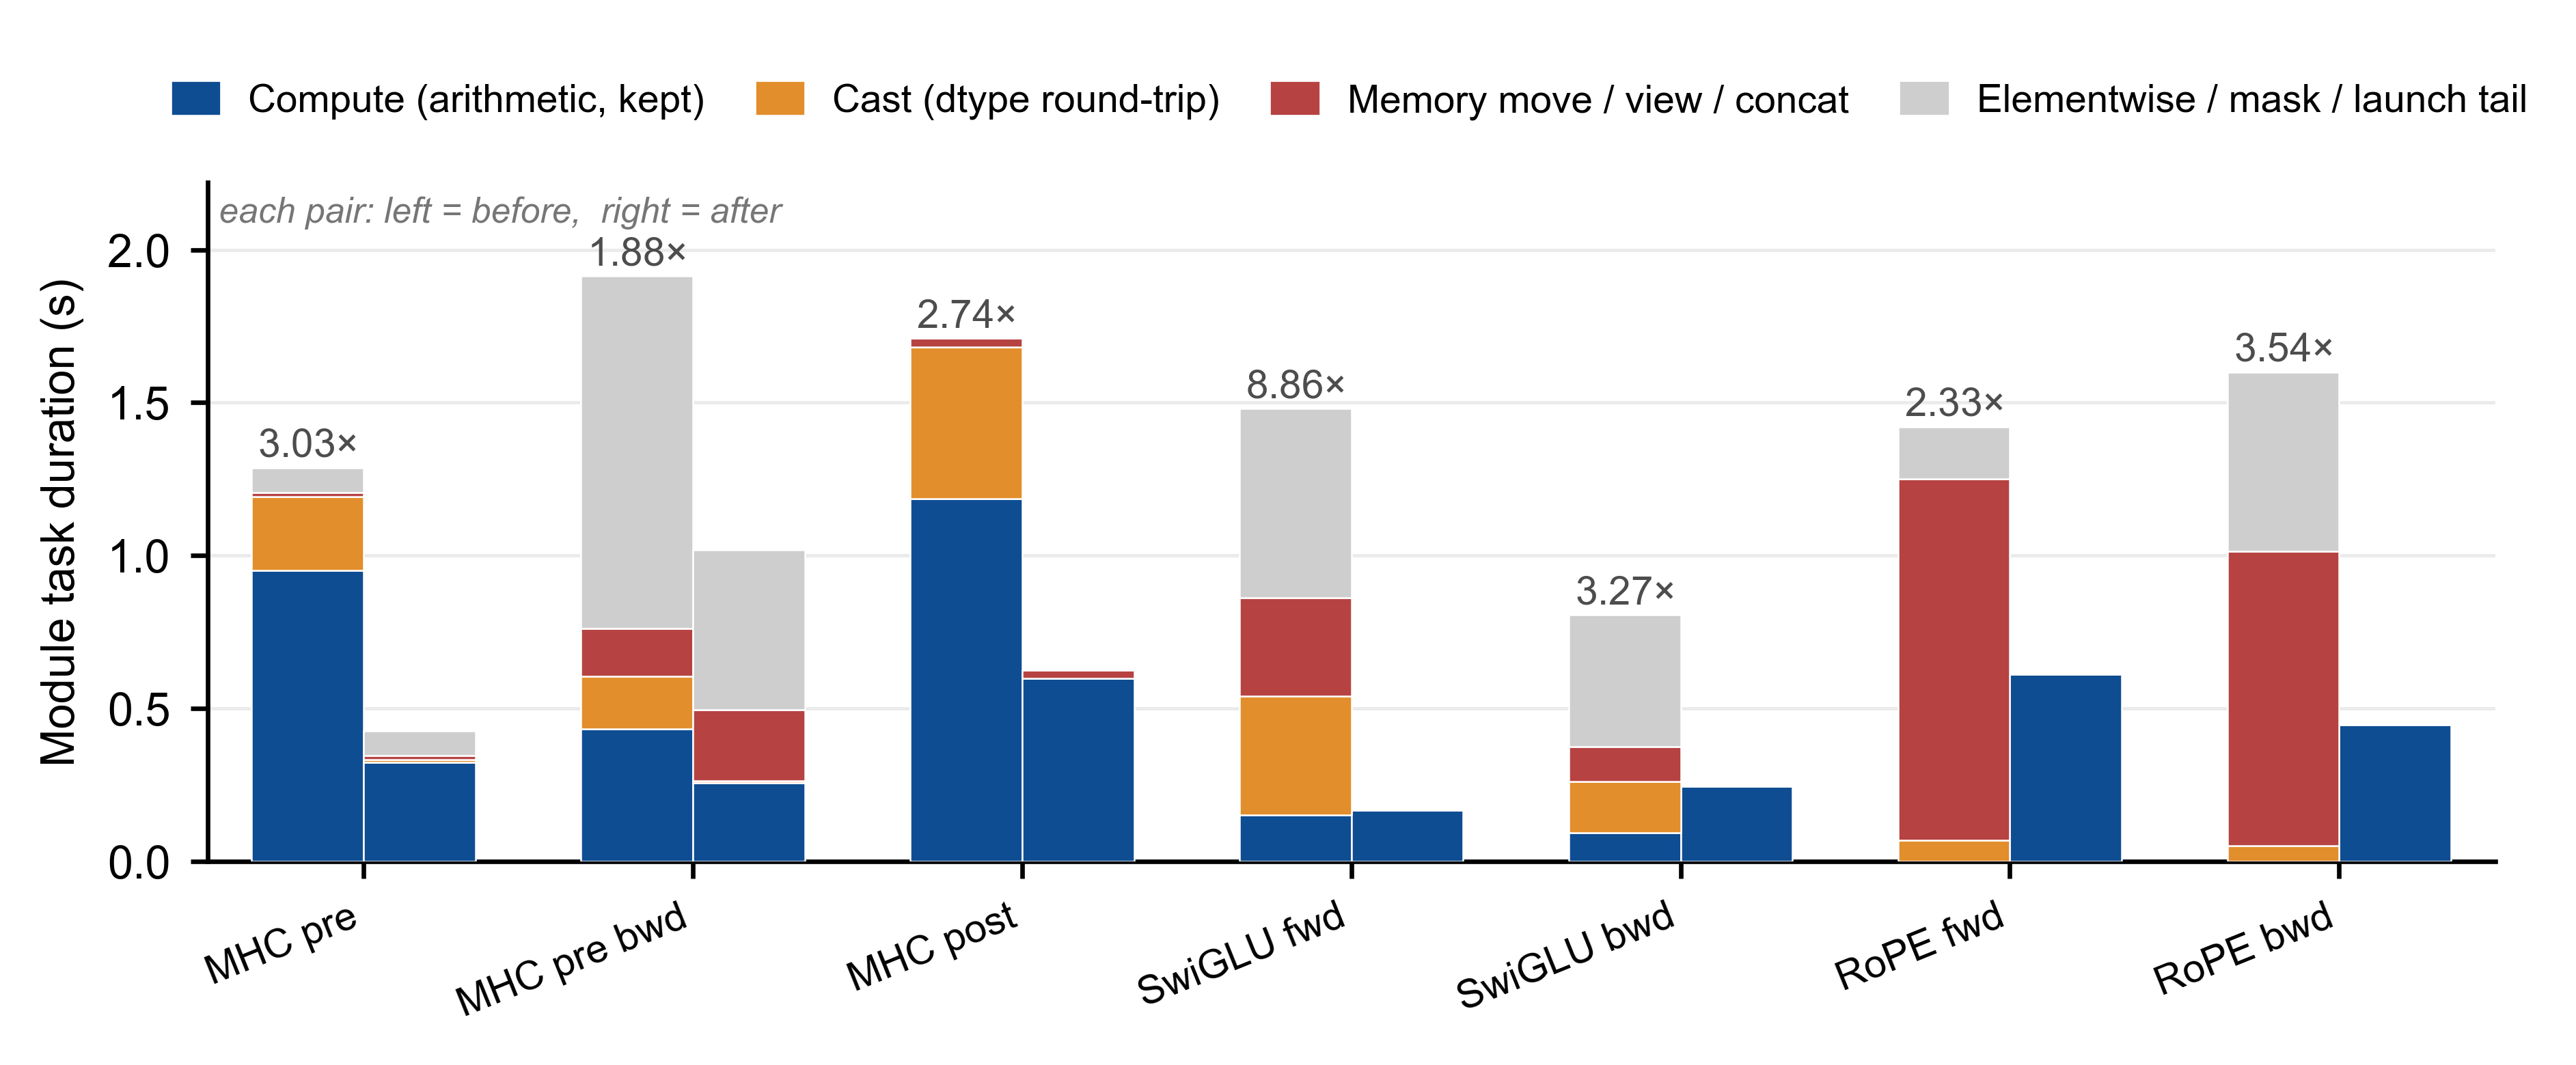
\includegraphics[width=0.92\textwidth]{figures/fig_fusion_time_breakdown.png}
\caption{Module task duration before (left bar) and after (right bar) operator fusion and rewrite for the seven targets, decomposed by operator category. Category durations are re-aggregated from the per-operator trace times of the pre- and post-optimization profiles. Each bar pair represents kernel-module durations~(Table~\ref{tab:operator_chain_fusion_results}), with the module speedup annotated above. Across targets, the baseline implementations are dominated by memory movement, dtype casts, and small elementwise/mask fragments, whereas the proposed fusion retain achieves significant efficiency improvements.}
\label{fig:fusion_time_breakdown}
\end{figure}

The mHC results exercise the two entries of this path together, so Table~\ref{tab:operator_chain_fusion_results} reports each stage separately. Pre-projection absorbs the RMS-normalization fragments and the original pre-BMM kernel; its backward absorbs the pre-BMM backward path, RMS backward fragments, casts, and elementwise reconstruction; and post-projection replaces the add/post-BMM1/cast portion. The three stages reach $3.03\times$, $1.88\times$, and $2.74\times$ at the module level (Table~\ref{tab:operator_chain_fusion_results}). This attribution is corroborated independently of the record counts: summing the inserted mHC fused kernels directly from the post-optimization trace reproduces the same stage totals, with \texttt{WindMhcPostPart} the single largest contributor at $0.313$\,s across all matched calls. The post-projection backward is left on its original path in this profile and is therefore not reported as a fused target, and folding it into the same boundary is left to future work.

Four of these kernels---the weight-free RMS normalization forward and backward and the pre-BMM contraction forward and backward---reach the AscendC substrate through the Triton rewrite rather than through eager-chain fusion, and comparing the original Triton kernel against its AscendC replacement at the single-operator level isolates what the substrate change alone contributes. Table~\ref{tab:triton_rewrite} reports this comparison. The RMS-normalization pair, measured at an identical BF16 shape, drops from $2307$\,\textmu s to $309$\,\textmu s forward ($7.48\times$) and from $3318$\,\textmu s to $439$\,\textmu s backward ($7.55\times$). Much of this comes from the tiling change, as the generic Triton kernel launches across $4096$ blocks whereas the AscendC kernel processes multiple rows per core across $48$ blocks. These ratios measure the Triton-to-AscendC rewrite against the original Triton kernel, and are therefore distinct from the AuraKernel figures in Section~\ref{subsec:eval_aurakernel} ($11.90\times$/$3.42\times$), which tune the resulting AscendC kernel further at a different shape. The pre-BMM contraction, whose rewrite also folds in the mixed-precision contract (FLOAT inputs become BF16), improves by $2.10\times$ forward and $1.89\times$ backward. The AIV pipeline decomposition confirms the affinity mechanism of Section~\ref{sec:kernel_fusion} rather than a mere clock reduction: on the pre-BMM forward the vector-compute ratio rises from $0.17$ to $0.86$ while the MTE2 load ratio falls from $0.59$ to $0.35$, so the \texttt{Brcb} broadcast and UB-resident contraction turn a movement-bound generic kernel into a vector-compute-dominated one. The same shift, in weaker form, appears on the backward kernels (pre-BMM backward vector ratio $0.14\rightarrow0.47$, RMS backward $0.28\rightarrow0.36$). Beyond these single-operator gains, the rewrite carries a stage-wide precision benefit that a generic Triton lowering left on the table: making the mixed-precision contract explicit removes a full-stage FP32 up-cast across the mHC pre-projection calls. Measured on the post-optimization trace, the \texttt{Cast} kernels of the stage fall from $241$\,ms to $8$\,ms in the forward path and from $172$\,ms to $6$\,ms in the backward path---about $400$\,ms of cast traffic removed across the combined stage, whose pre-optimization cost is $1.29$\,s forward plus $1.91$\,s backward---with a further $157$\,ms recovered from a backward \texttt{Mul} that the promotion had widened to FP32.

\begin{table}[h]
\centering
\caption{Triton-to-AscendC operator rewrite for the four mHC pre-projection kernels, measured as single-operator task duration at the profiled training shape. The RMS-normalization pair is compared at an identical BF16 input, while the pre-BMM pair additionally narrows its I/O dtype from FLOAT to BF16 as part of the rewrite. ``Vec.\ ratio'' is the duration-weighted AIV vector-compute ratio, whose rise on the AscendC side indicates a shift from movement-bound to compute-bound execution. Speedup is Triton/AscendC.}
\label{tab:triton_rewrite}
% \resizebox{\textwidth}{!}{%
\begin{tabular}{lccccc}
\toprule
\multirow{2}{*}{Kernel} & \multicolumn{2}{c}{Task duration (\textmu s)} & \multirow{2}{*}{Speedup} & \multicolumn{2}{c}{Vec.\ ratio} \\
\cmidrule(lr){2-3}\cmidrule(lr){5-6}
 & Triton & AscendC & & Triton & AscendC \\
\midrule
RMS-norm forward     & $2307$ & $309$ & $7.48\times$ & $0.30$ & $0.32$ \\
RMS-norm backward    & $3318$ & $439$ & $7.55\times$ & $0.28$ & $0.36$ \\
Pre-BMM forward      & $160$  & $76$  & $2.10\times$ & $0.17$ & $0.86$ \\
Pre-BMM backward     & $510$  & $270$ & $1.89\times$ & $0.14$ & $0.47$ \\
\bottomrule
\end{tabular}
% }
\end{table}

The remaining targets isolate the boundary-fusion effect, where autograd-visible tensor boundaries disappear. Limited SwiGLU forward collapses its eager clamp-and-gate chain into a single \texttt{SwiGluLimitV2} call, cutting the module from $1.480$\,s to $0.167$\,s ($8.86\times$), because the eager forward materialized clamp constants and a concatenation that the fused kernel keeps on chip. The backward path is more launch-dense still---fills, boolean materialization, selections, casts, \texttt{SwiGluGrad}, and concatenation---and there the fused \texttt{SwiGluLimitBackwardV2} operator removes almost the entire chain (Figure~\ref{fig:fusion_trace_schematic}). In the MoE path the same kernel also absorbs the routing-weight gradient, so the eager reduction that formed it (a full-size $\ell\cdot h$ product of $61$\,ms plus a \texttt{ReduceSum} of $20$\,ms per step, about $82$\,ms together) disappears into the fused pass at no added kernel cost. Counting the routing-gradient chain as part of the backward, the module falls from $805$\,ms to $246$\,ms ($3.27\times$). RoPE retains a larger optimized residual because the rewritten path still contains shape and indexing support operators, but the count accounting in Table~\ref{tab:operator_chain_fusion_results} exposes the same mechanism, yielding $2.33\times$ (forward) and $3.54\times$ (backward). The backward gain is the larger of the two because the fused kernel removes the eager slice-assignment scatter chain at the graph level. These module-level figures aggregate the query, key-value, and output sites.

These results close the loop with the bottleneck anatomy in Section~\ref{sec:kernel_bottleneck}. The gains are not explained by faster arithmetic alone, as Figure~\ref{fig:fusion_time_breakdown} makes explicit: they come from changing which tensors are materialized, which boundaries are visible to autograd, which dtype crosses global memory, and---for the Triton-originated stages---which substrate the arithmetic runs on. This is why the strongest effects appear on chains dominated by movement, conversion, and writeback rather than on compute-dense cube kernels, why the resource-utilization shift on the rewritten kernels turns scalar- and movement-bound loops into vector-compute-dominated ones, and why the appropriate baseline is the emitted trace slice, stage subgraph, or generic Triton kernel rather than an isolated primitive operator.


\subsection{Long-term Training Stability with Ascend SuperPOD}
\label{subsec:npu_training_stability}

Stable training is a prerequisite for meaningful downstream evaluation. If the training process is unstable, subsequent benchmark differences become difficult to interpret. In this work, we implement stable SFT training of DeepSeek-V4-Flash in a Ascend-based environment with 8 nodes and 128 Ascend 910C NPUs in total.

Using the 50K self-distilled dataset as an example, we complete a relatively full-scale SFT verification run on DeepSeek-V4-Flash. The training configuration uses \texttt{GBS=128}, \texttt{MBS=1}, and \texttt{SEQ\_LEN=8192}. The model is trained for \texttt{800} steps, and checkpoints are saved at \texttt{200}, \texttt{400}, \texttt{600}, and \texttt{800} steps. The training log shows that the job successfully reaches \texttt{iteration 800/800}, without skipped iterations or NaN iterations. At the final iteration, the \texttt{lm loss} converges to approximately \texttt{0.079}, the \texttt{mtp\_1 loss} is approximately \texttt{0.093}, and the gradient norm remains within a normal range. The overall training curve decreases continuously and then gradually becomes stable.

As shown in Figure~\ref{fig:sft_50k_stability}, these observations indicate that the current data preprocessing pipeline, MindSpeed-LLM~\citep{mindspeed-llm} training script, DeepSeek-V4-Flash base model, and 8-node 910C training environment form a reproducible and sustainable full-parameter SFT workflow. This provides a stable foundation for subsequent experiments on different data scales, data mixtures, and task-oriented data-distillation strategies.

\begin{figure}[t]
\centering
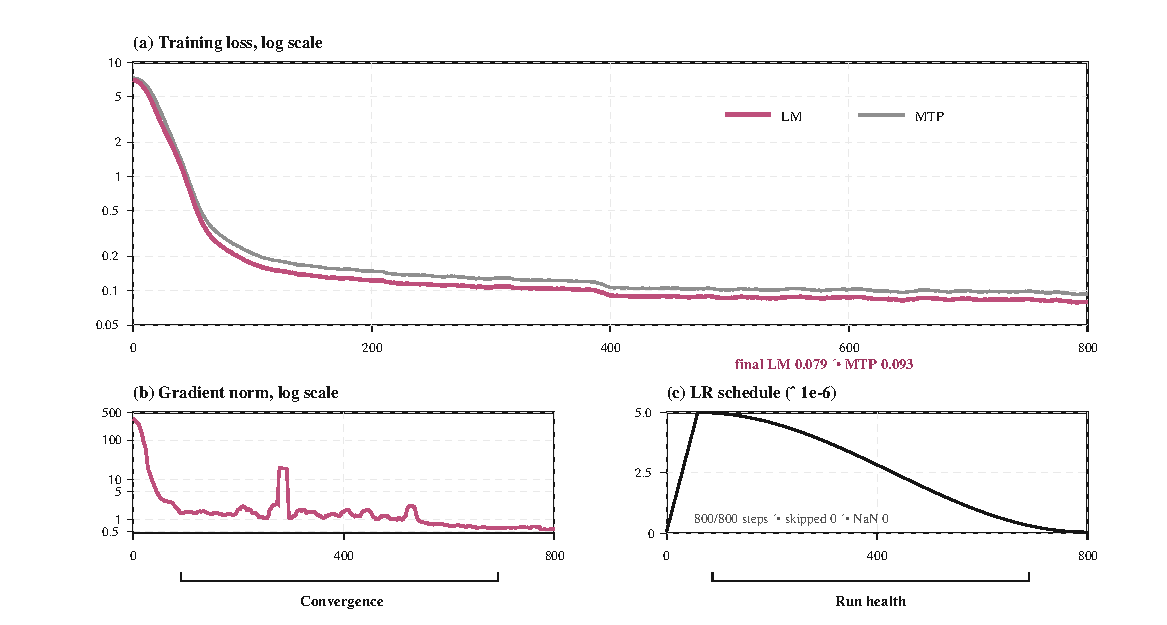
\includegraphics[width=\linewidth]{figures/fig_50k_sft_stability_paper.pdf}
\caption{Training stability of the 50K self-distilled SFT run on Ascend 910C NPUs. The model is trained for 800 steps with \texttt{GBS=128}, \texttt{MBS=1}, and \texttt{SEQ\_LEN=8192}, and the training process reaches the final iteration without skipped or NaN iterations.}
\label{fig:sft_50k_stability}
\end{figure}

\subsection{SFT Scaling and Cleaning Analysis}
\label{subsec:sft_training_cleaning}


The first systematic experiments on 3K, 10K, and 50K self-distilled data show that SFT brings two opposite effects. On the one hand, SFT helps the model learn code-protocol tasks such as B4O-Feasible. Using DeepSeek-V4-Flash as the baseline, we find that B4O-Feasible improves from 60.47 to 65.07 with SFT-10K, and B4O-ORGEval improves from 34.26 to 47.21. These gains indicate that SFT makes the model more familiar with code-only output, \texttt{data.json} loading, Gurobi model construction, LP writing paths, and other benchmark-specific protocols, with the strongest relative improvement concentrated on structural-equivalence evaluation.

On the other hand, SFT also weakens part of the model's original ability on natural-language modeling tasks. The baseline obtains 84.08 on NL4OPT, while SFT-10K obtains 81.66. Similarly, the baseline obtains 63.33 on OptiBench, while SFT-10K obtains 62.67. Further scaling to 50K does not solve this issue; instead, OptiBench decreases to 58.68. Since the 3K, 10K, and 50K settings follow almost the same construction design, the degradation of 50K is difficult to explain as a data-mixture change. A more plausible explanation is that continuous iterative distillation introduces lower-quality samples and amplifies the model's own noise.


\begin{table}[t]
\centering
\small
\caption{Systematic comparison of SFT data scales on OR modeling benchmarks.}
% \resizebox{\textwidth}{!}
% {
\begin{tabular}{lcccc}
\toprule
Model & NL4OPT & OptiBench & B4O-Feasible & B4O-ORGEval \\
\midrule
DeepSeek-V4-Flash & 84.08 & 63.33 & 60.47 & 34.26 \\
SFT-3K  & 80.62 & 60.66 & 64.51 & 43.65 \\
SFT-10K & 81.66 & 62.67 & 65.07 & 47.21 \\
SFT-50K & 82.01 & 58.68 & 64.97 & 45.94 \\
\bottomrule
\end{tabular}
% }

\label{tab:sft_scale}
\end{table}


Table~\ref{tab:sft_scale} supports two observations. First, supervised fine-tuning provides a clear benefit for protocol-oriented OR modeling tasks: all SFT variants improve B4O-Feasible and, more prominently, B4O-ORGEval relative to the base model, indicating that the self-distilled data contains effective supervision for solver-facing output formats and benchmark-specific conventions. Second, the gains are not monotonic with data scale. If additional self-distilled samples were uniformly beneficial, SFT-50K would be expected to dominate SFT-10K, and the uncleaned SFT-10K checkpoint would not fall below the base model on NL4OPT and OptiBench. The observed regressions suggest that scaling the same self-distillation pipeline also increases the weight of weakly verified or biased samples. Such samples can reinforce useful modeling patterns, but they can also amplify systematic errors inherited from the base model. Therefore, the 50K result should be interpreted less as evidence against SFT scale itself and more as evidence that scale must be coupled with stronger verification and data-quality control. This motivates returning to the 10K setting for fine-grained cleaning rather than further expanding the unfiltered pipeline to 100K.

The SFT results after cleaning validate the effectiveness of the contract-aware cleaning and CoT enhancement framework introduced in Section~\ref{subsec:sft_cot_cleaning}. Compared with the uncleaned SFT-10K, Clean-CoT improves NL4OPT by 5.27 percentage points, OptiBench by 1.50 percentage points, B4O-Feasible by 0.86 percentage points, and B4O-ORGEval by 1.52 percentage points. This result suggests that the main issue of the 10K data is not insufficient scale, but semantic noise that is strong enough to damage natural-language modeling ability. Once such noise is systematically filtered and repaired, SFT no longer harms NL4OPT and OptiBench, but instead outperforms both the baseline and the original SFT-10K while further improving both B4O metrics.


\begin{table}[t]
\centering
\small
\caption{Effect of data cleaning and CoT enhancement on OR modeling benchmarks.}
% \resizebox{\textwidth}{!}{
\begin{tabular}{lcccc}
\toprule
Model & NL4OPT & OptiBench & B4O-Feasible & B4O-ORGEval \\
\midrule
DeepSeek-V4-Flash & 84.08 & 63.33 & 60.47 & 34.26 \\
SFT-10K & 81.66 & 62.67 & 65.07 & 47.21 \\
SFT-Clean-only & 84.23 & 63.08 & 64.31 & 48.28 \\
SFT-Clean-CoT & \textbf{86.93} & \textbf{64.17} & \textbf{65.93} & \textbf{48.73} \\
\bottomrule
\end{tabular}
% }

\label{tab:sft_cleaning}
\end{table}

However, the gains of Clean-CoT are not uniformly distributed across all tasks. It is most effective on NL4OPT and OptiBench because these targets allow \texttt{<think>}, \texttt{<model>}, and \texttt{<python>} style answers. The structured modeling checklist can directly enter the training response and help the model learn explicit judgments about variable domains, objective direction, and constraint direction. By contrast, B4O-Feasible and B4O-ORGEval are code-only tasks, where explanatory chain-of-thought cannot appear in the output. Therefore, the advantage of Clean-CoT is less directly expressed in the response format. In the updated results, Clean-CoT also outperforms clean-only on B4O-Feasible (65.93 vs.\ 64.31) and B4O-ORGEval (48.73 vs.\ 48.28), but the margins are smaller than on NL4OPT. This suggests that CoT-oriented enhancement is beneficial for code-only tasks, yet these tasks still require more specialized training on schema reading, index alignment, variable-family design, \texttt{model.write()} paths, and LP-structure consistency.


Error analysis further reveals the boundary of cleaning-based enhancement. On NL4OPT, Clean-CoT reduces \texttt{wrong\_objective\_or\_model} errors from 52 cases before cleaning to 31 cases. On OptiBench, the same error type decreases from 154 to 128 cases, indicating that modeling checklists indeed reduce coarse errors at the objective and constraint levels. However, \texttt{nonlinear\_or\_bad\_gurobi\_form} errors on OptiBench do not decrease; instead, they increase from 49 to 56 cases. This shows that ordinary cleaning and short chain-of-thought enhancement can improve the question of what model should be built, but are insufficient to stably solve the question of how to correctly express nonlinear terms, ratios, averages, and quadratic terms in Gurobi. This observation motivates the subsequent design of nonlinear repair and specialized nonlinear/Gurobi synthetic data, rather than forcing all issues into a single Clean-CoT path.

Therefore, the main conclusion of this SFT experiment is that chain-of-thought-oriented data enhancement is effective, but it must be constrained, contract-aware, and gated by reviewer and validation checks. Its value is not to make the model generate longer reasoning, but to inject the most error-prone optimization-modeling checkpoints into the training distribution in a stable form.

\subsection{Effect of CPT Initialization under Matched SFT Conditions}
\label{subsec:cpt_sft_transfer}

Following the evaluation protocol in Section~\ref{subsubsec:cpt_checkpoint_selection}, we evaluate whether the CPT checkpoint improves downstream SFT performance under matched SFT conditions. Both the direct SFT route and the CPT-initialized SFT route use the same 10K chain-of-thought OR modeling samples, 220 SFT iterations, peak learning rate \(5\times10^{-6}\) with cosine decay, global batch size 128, and sequence length 8192. Therefore, performance differences between the two routes can be attributed to CPT initialization rather than different SFT data or optimization settings.

We report results on four OR benchmarks. NL4OPT and OptiBench evaluate natural-language optimization modeling, B4O-Feasible evaluates whether the generated Gurobi program executes successfully and produces a feasible solution, and B4O-ORGEval evaluates whether the generated optimization model is structurally equivalent to the reference model, independent from implementations. Table~\ref{tab:cpt_sft_transfer} 
shows that SFT alone is already a strong baseline. Compared with the base model, direct SFT improves NL4OPT from 84.08\% to 86.93\%, OptiBench from 63.33\% to 64.17\%, B4O-Feasible from 60.47\% to 65.93\%, and B4O-ORGEval from 34.26\% to 48.73\%. This confirms that the 10K CoT OR modeling samples provide effective task-level supervision for activating optimization modeling capabilities.

\begin{table}[t]
\centering
\small
\caption{CPT-to-SFT transfer results on four OR modeling benchmarks.}
% \resizebox{\textwidth}{!}{
\begin{tabular}{lcccc}
\toprule
Model & NL4OPT & OptiBench & B4O-Feasible & B4O-ORGEval \\
\midrule
DeepSeek-V4-Flash
    & 84.08 & 63.33 & 60.47 & 34.26 \\
SFT-Clean-CoT
    & 86.93 & 64.17 & 65.93 & 48.73 \\
CPT+SFT-Clean-CoT
    & \textbf{89.52} & \textbf{67.12} & \textbf{71.22} & \textbf{59.39} \\
\bottomrule
\end{tabular}
% }

\label{tab:cpt_sft_transfer}
\end{table}


CPT initialization provides further gains on top of this SFT baseline across all four benchmarks: +2.59 pp on NL4OPT, +2.95 pp on OptiBench, +5.29 pp on B4O-Feasible, and +10.66 pp on B4O-ORGEval. The gain is present on both executability and structure but is largest on B4O-ORGEval, indicating that CPT supplies OR-domain modeling priors that improve solver-facing feasibility and, most strongly, structural equivalence---capabilities that matched-condition SFT alone does not fully activate.

Since B4O-ORGEval emphasizes mathematical equivalence between the generated and reference optimization models, it is more directly aligned with the domain knowledge and modeling patterns introduced during CPT.

Overall, these results support the value of domain-adaptive CPT as a preparation stage for OR-oriented SFT. While direct SFT already improves task performance, CPT further strengthens the structurally demanding capabilities required for optimization model equivalence. This motivates scaling CPT with broader OR task coverage, higher-quality solver-verified documents, and retention-aware data mixtures in future experiments.


\subsection{Performance of the Proposed Post-Training Pipeline}

\textbf{Evaluation Setup.} We evaluate on four OR benchmarks---NL4OPT~\citep{ramamonjison2023nl4opt} and OptiBench~\citep{yang2025optibench} for natural-language optimization modeling and problem understanding, B4O-Feasible for executability, and B4O-ORGEval for structural equivalence~\citep{orgeval}---alongside general benchmarks MMLU~\citep{hendryckstest2021}, MMLU-Pro~\citep{wang2024mmlu}, CMMLU~\citep{hendryckstest2021}, HumanEval~\citep{chen2021codex}, GSM8K~\citep{cobbe2021gsm8k}, and MATH~\citep{hendrycks2021measuringmathematicalproblemsolving} (Table~\ref{tab:ours_vs_base_general}). For decoding, we use greedy for Pass@1 and sample at $T=0.8$ with top-$p=0.95$ for Pass@4, applying unbiased estimation~\citep{zhao2023unbiased}. Correctness for B4O-Feasible requires runtime execution and contract adherence; B4O-ORGEval uses the ORGEval WL reward on the normalized formulation graph to measure semantic structural match. All evaluations share the same prompt template and decoding budget for fair comparison.


While SFT improves extraction tasks, structural equivalence, and zero-shot B4O-Feasible performance, it does not consistently enhance executability across all decoding settings; the 5-shot B4O-Feasible result remains below the base model. The full CPT+SFT pipeline consistently improves 0-shot Pass@1 across the OR benchmarks and yields its strongest gains on B4O-ORGEval (structural equivalence) and B4O-Feasible (executability), but it should not be interpreted as dominating every decoding regime. This indicates that CPT supplies domain knowledge critical for both deep structural reasoning and the generation of executable code, while SFT aligns outputs with format and protocol requirements.


\begin{table*}[t!]
\centering
\caption{Performance of Base, SFT, and CPT+SFT models on operations research benchmarks. The SFT model and the SFT stage of CPT+SFT both use the Clean‑CoT dataset. All numbers are percentages. The best result in each column is in \textbf{bold}, and the second best is \underline{underlined}. Gains are absolute differences (percentage points) compared to the Base model. }
\label{tab:main_results}
\small
\setlength{\tabcolsep}{12pt}
\resizebox{\textwidth}{!}{
\begin{tabular}{llcccccc}
\toprule
\multirow{2}{*}{Dataset} & \multirow{2}{*}{Model} & \multicolumn{2}{c}{0-shot Pass@1} & \multicolumn{2}{c}{0-shot Pass@4} & \multicolumn{2}{c}{5-shot Pass@1} \\
\cmidrule(lr){3-4} \cmidrule(lr){5-6} \cmidrule(lr){7-8}
                        &                       & Value & Gain & Value & Gain & Value & Gain \\
\midrule
\multirow{3}{*}{NL4OPT} & \hspace{1em} \texttt{Base}      & 84.08           & ---   & 91.35           & ---   & 88.24           & ---   \\
                        & \hspace{1em} \texttt{SFT}       & \underline{86.93}& +2.85 & \underline{92.39}& +1.04 & \underline{88.97}& +0.73 \\
                        & \hspace{1em} \texttt{CPT+SFT}   & \textbf{89.52}  & \textcolor{slai}{+5.44} & \textbf{93.15}  & \textcolor{slai}{+1.80} & \textbf{90.66}  & \textcolor{slai}{+2.42} \\
\cmidrule(lr){1-8}
\multirow{3}{*}{OptiBench} & \hspace{1em} \texttt{Base}    & 63.33           & ---   & \underline{72.50}& ---   & \underline{66.00}& ---   \\
                            & \hspace{1em} \texttt{SFT}     & \underline{64.17}& +0.84 & 71.50           & -1.00 & 65.67           & -0.33 \\
                            & \hspace{1em} \texttt{CPT+SFT} & \textbf{67.12}  & \textcolor{slai}{+3.79} & \textbf{72.83}  & \textcolor{slai}{+0.33} & \textbf{66.89}  & \textcolor{slai}{+0.89} \\
\cmidrule(lr){1-8}
\multirow{3}{*}{B4O-Feasible} & \hspace{1em} \texttt{Base}   & 60.47           & ---   & 66.86           & ---   & \textbf{78.20}  & ---   \\
                              & \hspace{1em} \texttt{SFT}    & \underline{65.93}& +5.46 & \underline{68.69}& +1.83 & 73.55           & -4.65 \\
                              & \hspace{1em} \texttt{CPT+SFT}& \textbf{71.22}  & \textcolor{slai}{+10.75} & \textbf{82.41}  & \textcolor{slai}{+15.55}& \underline{74.78}& -3.42 \\
\cmidrule(lr){1-8}
\multirow{3}{*}{B4O-ORGEval} & \hspace{1em} \texttt{Base}    & 34.26           & ---   & 49.49           & ---   & 71.57           & ---   \\
                             & \hspace{1em} \texttt{SFT}     & \underline{48.73}& +14.47& \underline{56.35}& +6.86 & \underline{82.99}& +11.42\\
                             & \hspace{1em} \texttt{CPT+SFT} & \textbf{59.39}  & \textcolor{slai}{+25.13} & \textbf{67.28}  & \textcolor{slai}{+17.79} & \textbf{84.52}  & \textcolor{slai}{+12.95} \\
\bottomrule
\end{tabular}}
\end{table*}

To evaluate the complementary roles of knowledge injection and instruction tuning, we conduct end-to-end experiments comparing Base, SFT, and CPT+SFT under identical SFT conditions. Our central hypothesis is that CPT supplies domain-specific structural priors, while SFT grounds execution protocols and format compliance. The results in Table~\ref{tab:main_results} confirm that the full pipeline (CPT+SFT) consistently outperforms both Base and SFT across all OR benchmarks in 0-shot Pass@1. The gain is largest on B4O-ORGEval (e.g., +10.66 pp in 0-shot Pass@1 and +7.71 pp in the three-setting mean over SFT) and is also substantial on B4O-Feasible (+5.29 pp in 0-shot Pass@1 and +6.75 pp in the three-setting mean over SFT). SFT alone improves B4O-Feasible in zero-shot settings but drops below Base in 5-shot, indicating that instruction tuning by itself is insufficient to stabilize executability across prompting regimes.

\begin{figure}[t!]
    \centering
    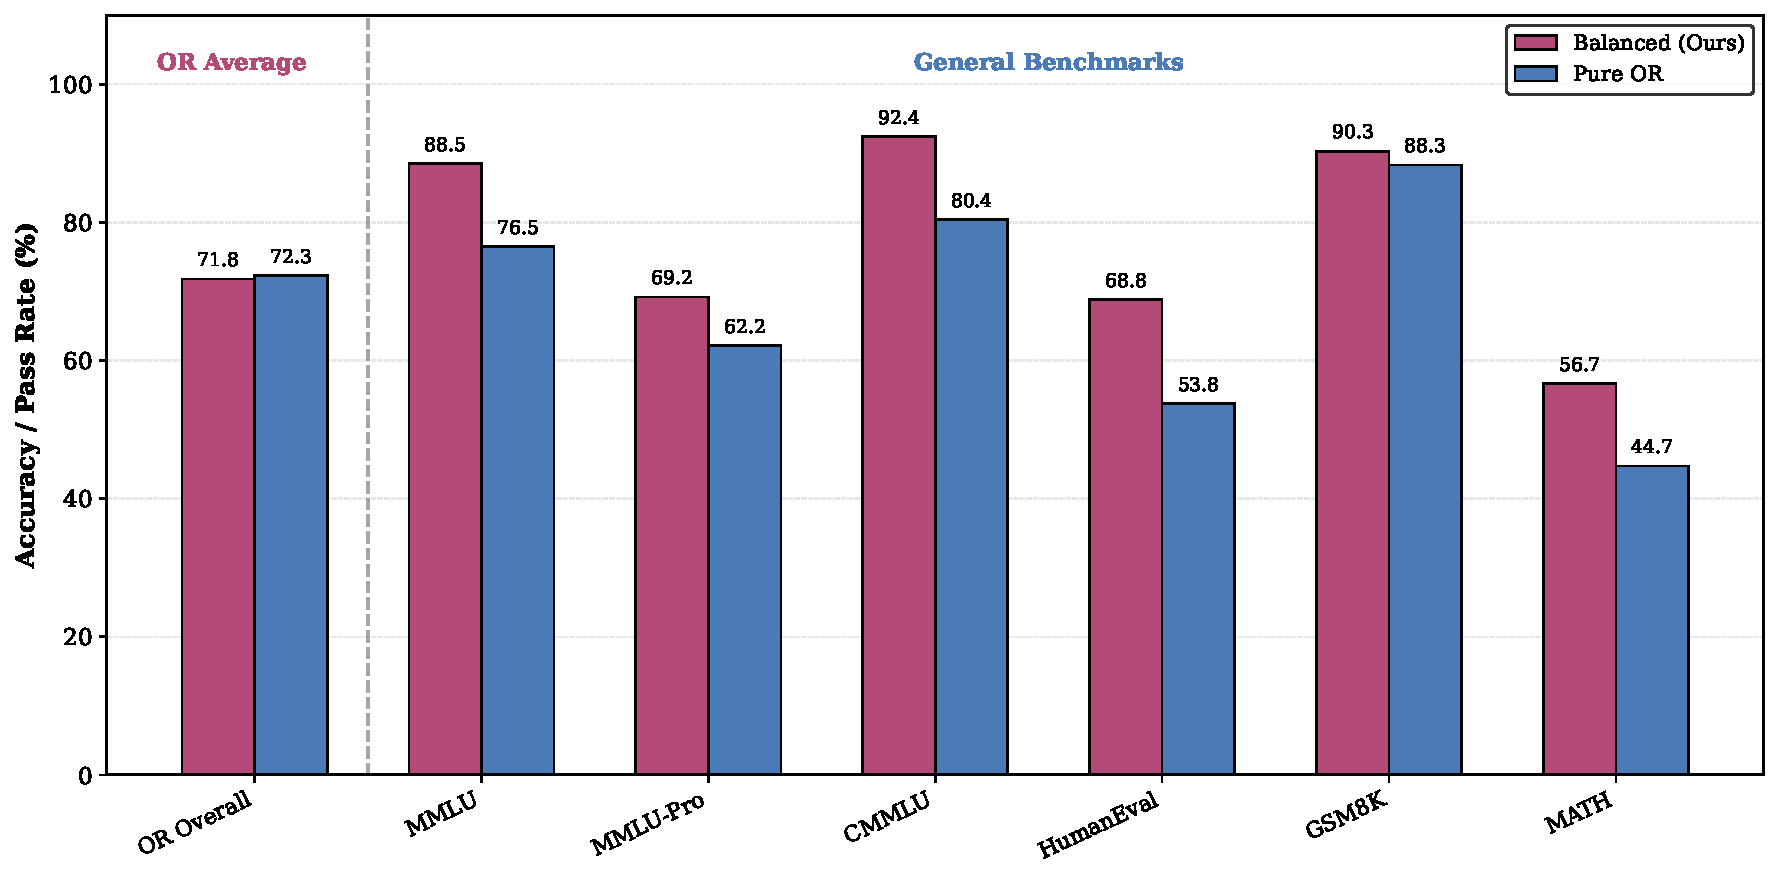
\includegraphics[width=0.9\textwidth]{figures/ablation.pdf}
    \caption{
        Ablation on data mixture under the end‑to‑end (CPT$\to$SFT) pipeline.
        % Comparison between Balanced (our configuration, with both OR and general data) and Pure OR (CPT trained exclusively on operations research data).
        % While Pure OR causes a drastic drop (10–15 points) on general benchmarks (MMLU~\citep{hendryckstest2021}, CMMLU~\citep{hendryckstest2021}~\citep{hendryckstest2021}, MMLU~\citep{hendryckstest2021}-PRO, HumanEval~\citep{chen2021codex}, GSM8K~\citep{cobbe2021gsm8k}, MATH~\citep{hendrycks2021measuringmathematicalproblemsolving}), it yields no improvement on OR Overall—even slightly underperforming Balanced due to measurement noise.
        % This confirms that interleaving domain and general data during CPT is essential to inject structural priors without sacrificing broad reasoning capabilities.
    }
    \label{fig:ablation}
\end{figure}


\begin{table*}[t]
\centering
\caption{Performance comparison between Ours and Base on general benchmarks.}
\label{tab:ours_vs_base_general}
\small
\setlength{\tabcolsep}{22pt}
\resizebox{\textwidth}{!}{
\begin{tabular}{llccc}
\toprule
\multirow{2}{*}{Category} & \multirow{2}{*}{Benchmark} & \multirow{2}{*}{\# Shots} & \multicolumn{2}{c}{Model}\\
\cmidrule(lr){4-5}
& & & \textbf{\modelname (Ours)} & Base \\
\midrule
             & MMLU~\citep{hendryckstest2021} & 5-shot & 88.5 (+0.9) & 87.6 \\
World Knowledge & MMLU-Pro~\citep{wang2024mmlu} & 5-shot & 69.2 (-1.8) & 71.0 \\
             & CMMLU~\citep{hendryckstest2021} & 5-shot & 92.4 (+0.3) & 92.1 \\
\midrule
             & HumanEval~\citep{chen2021codex} & 0-shot & 68.8 (-0.6) & 69.4 \\
Code \& Math & GSM8K~\citep{cobbe2021gsm8k} & 8-shot & 90.3 (+0.5) & 89.8 \\
             & MATH~\citep{hendrycks2021measuringmathematicalproblemsolving} & 4-shot & 56.7 (-1.7) & 58.4 \\
\bottomrule
\end{tabular}}
\end{table*}


\begin{table}[t!]
\centering
\caption{Performance of various models on operations research benchmarks. The best result in each column is in \textbf{bold}, and the second best is \underline{underlined}.}
\label{tab:models_or}
\small
\setlength{\tabcolsep}{5pt}
\resizebox{\textwidth}{!}
{
\begin{tabular}{lccccc}
\toprule
\multirow{2}{*}{Model} & \multicolumn{4}{c}{Operations Research Benchmarks} & \multirow{2}{*}{Overall}\\
\cmidrule(lr){2-5}
& NL4OPT & OptiBench & B4O-Feasible & B4O-ORGEval\\
\midrule
GLM-5.2~\citep{glm5team2026glm5vibecodingagentic}               & 78.55 & 55.33 & 61.05 & 31.47 & 56.60 \\
DeepSeek-V4-Flash~\citep{deepseekai2026deepseekv4highlyefficientmilliontoken}     & 84.08 & 63.33 & 60.47 & 34.26 & 60.54 \\
MiMo-V2.5-Pro~\citep{mimo2026v25pro}         & 80.97 & 56.83 & 70.35 & 41.88 & 62.51 \\
Kimi-K2.6~\citep{kimiteam2026kimik2openagentic}             & 78.89 & 59.83 & \underline{72.67} & \underline{46.95} & 64.59 \\
Gemini-3-Flash~\citep{google_gemini_flash}        & 79.93 & \textbf{68.83} & 71.80 & 46.70 & 66.82 \\
GPT-5.4-Mini~\citep{openai_gpt_5_4_mini}         & \underline{87.89} & 66.17 & \textbf{73.84} & 43.40 & \underline{67.83} \\
\textbf{\modelname~(Ours)}                  & \textbf{89.52} & \underline{67.12} & 71.22 & \textbf{59.39} & \textbf{71.81} \\
\bottomrule
\end{tabular}
}
\end{table}


Disaggregating by task type reveals the distinct contributions of each stage. For structural equivalence tasks (B4O-ORGEval), SFT alone improves moderately over the base model, but the additional CPT prefix yields a substantial leap. This suggests that optimization modeling judgments---which require understanding mathematical intent independent of surface form---benefit from dense exposure to OR corpora during CPT, an exposure that SFT cannot fully replicate due to its instruction-focused, smaller-scale format. For code-execution and feasibility tasks (B4O-Feasible), SFT improves 0-shot Pass@1 and Pass@4 but remains below Base in 5-shot, yielding only a modest three-setting mean gain (69.39 vs.\ 68.51), whereas CPT+SFT reaches 76.14. This suggests that domain-specific pretraining is crucial for generating executable optimization code, beyond what format and protocol alignment alone can provide. On general benchmarks (Table~\ref{tab:ours_vs_base_general}), CPT+SFT achieves performance comparable to Base, with slight fluctuations in both directions (e.g., +0.9 on MMLU~\citep{hendryckstest2021}, -1.7 on MATH~\citep{hendrycks2021measuringmathematicalproblemsolving}), and no signs of catastrophic forgetting. This confirms that the staged data mixture (\textasciitilde 75\% OR + retained general corpora) preserves broad reasoning capabilities. As shown in Table~\ref{tab:models_or}, our CPT+SFT model attains the highest overall score across all four OR benchmarks, outperforming strong baselines such as GPT-5.4-Mini~\citep{openai_gpt_5_4_mini} and Gemini-3-Flash~\citep{google_gemini_flash} by a substantial margin.


To dissect the sources of CPT's effectiveness, we ablate the CPT data mixture under the same end-to-end pipeline (Figure~\ref{fig:ablation}). We compare two configurations: Balanced (our mixture of OR and general data) and Pure OR (only OR data). As shown, Pure OR causes a drastic drop (10–15 points) on general benchmarks while yielding no improvement on OR Overall compared to Balanced---in fact, it slightly underperforms Balanced. This indicates that exclusive domain pretraining leads to overfitting that harms general capabilities without benefiting domain performance. In contrast, Balanced achieves strong results on both OR and general benchmarks, demonstrating that interleaving domain-specific and general data during CPT is essential to inject structural priors while retaining broad reasoning abilities and guarding against catastrophic forgetting.

In summary, the end-to-end experiments show a complementary pattern between
SFT and CPT. SFT establishes supervised task alignment and protocol-oriented
output behavior, while CPT supplies domain-structural priors that drive the
largest additional gains, most clearly on B4O-ORGEval and also on
B4O-Feasible. Together, the two stages form a complementary pipeline for
improving OR-domain performance while preserving general capability.


% Having established the optimal training configuration, we next evaluate whether the agentic inference pipeline can further leverage this model to correct residual reasoning errors at test time.


% \subsection{Inference-Mode Agentic Rollout Evaluation}
% \label{subsec:agent_inference_eval}

% We evaluate the four-stage agentic rollout pipeline in pure inference
% mode, with no RL training applied at any stage. All rollouts use
% DeepSeek-V4-Flash~\citep{xu2026deepseek} served via vLLM on Ascend 910C NPUs, evaluated on
% OptiBench. A solution is marked correct if the generated Gurobi code
% reaches \texttt{OPTIMAL} status and its \texttt{model.ObjVal} matches
% the ground-truth reference within a relative tolerance of $10^{-6}$.
% We report results for four configurations: the base model and clean-cot
% SFT checkpoint, each with and without the four-stage agent. Failures are
% classified into three categories via LLM-assisted post-hoc analysis:
% \texttt{code\_error} (execution failure due to syntax errors, runtime
% exceptions, or solver infeasibility introduced by the code),
% \texttt{code\_mismatch} (code reaches \texttt{OPTIMAL} but does not
% faithfully implement the formulation), and \texttt{modeling\_error}
% (the formulation is conceptually wrong and the code implements it
% correctly). Table~\ref{tab:fine_grained_failure} reports aggregate
% results; Table~\ref{tab:transitions} shows per-sample category
% transitions across three configuration pairs.

% \begin{table}[t]
% \centering
% \small
% \caption{Inference-mode accuracy and fine-grained failure
% classification on OptiBench.}
% \begin{tabular}{lcccc}
% \toprule
% Configuration
%   & Accuracy
%   & \texttt{code\_error}
%   & \texttt{code\_mismatch}
%   & \texttt{modeling\_error} \\
% \midrule
% base model         & 63.33\% & 66 & 39  & 115 \\
% base model + agent & \textbf{72.17\%} & 15 & 59  & 93  \\
% clean-cot          & 66.17\% & 74 & 39  & 90  \\
% clean-cot + agent  & 69.67\% & 20 & 53  & 109 \\
% \bottomrule
% \end{tabular}
% \label{tab:fine_grained_failure}
% \end{table}

% \begin{table*}[t]
% \centering
% \small
% \caption{Per-sample failure category transitions across three
% configuration pairs. Each cell gives the number of problems whose
% category changed from the row label (source) to the column label
% (target). Row totals for failure categories equal the source
% configuration count for that category; row total for \emph{correct}
% equals the number of regressions. \emph{correct}: solved in that
% configuration.}
% \label{tab:transitions}

% \begin{subtable}[t]{\linewidth}
% \centering
% \caption{base model $\to$ clean-cot}
% \begin{tabular}{lrrrrr}
% \toprule
% & \multicolumn{4}{c}{Target} & \\
% \cmidrule{2-5}
% Source & correct & code\_error & code\_mismatch & modeling\_error & Total \\
% \midrule
% correct         & --  & 14 &  2 & 10 &  26 \\
% code\_error     &  8  & 45 &  2 & 11 &  66 \\
% code\_mismatch  &  9  &  4 & 19 &  7 &  39 \\
% modeling\_error & 26  & 11 & 16 & 62 & 115 \\
% \midrule
% Total           & 43  & 74 & 39 & 90 &  -- \\
% \bottomrule
% \end{tabular}
% \end{subtable}

% \vspace{6pt}

% \begin{subtable}[t]{\linewidth}
% \centering
% \caption{base model $\to$ base model + agent}
% \begin{tabular}{lrrrrr}
% \toprule
% & \multicolumn{4}{c}{Target} & \\
% \cmidrule{2-5}
% Source & correct & code\_error & code\_mismatch & modeling\_error & Total \\
% \midrule
% correct         & --  &  2 &  6 &  8 &  16 \\
% code\_error     & 22  & 10 & 20 & 14 &  66 \\
% code\_mismatch  & 14  &  0 & 18 &  7 &  39 \\
% modeling\_error & 33  &  3 & 15 & 64 & 115 \\
% \midrule
% Total           & 69  & 15 & 59 & 93 &  -- \\
% \bottomrule
% \end{tabular}
% \end{subtable}

% \vspace{6pt}

% \begin{subtable}[t]{\linewidth}
% \centering
% \caption{clean-cot $\to$ clean-cot + agent}
% \begin{tabular}{lrrrrr}
% \toprule
% & \multicolumn{4}{c}{Target} & \\
% \cmidrule{2-5}
% Source & correct & code\_error & code\_mismatch & modeling\_error & Total \\
% \midrule
% correct         & --  &  5 &  3 & 20 &  28 \\
% code\_error     & 26  & 11 & 17 & 20 &  74 \\
% code\_mismatch  &  6  &  0 & 23 & 10 &  39 \\
% modeling\_error & 17  &  4 & 10 & 59 &  90 \\
% \midrule
% Total           & 49  & 20 & 53 & 109 & -- \\
% \bottomrule
% \end{tabular}
% \end{subtable}

% \end{table*}

% The transition matrix for base model $\to$ base model + agent shows
% that 56 of the 66 \texttt{code\_error} cases leave that category: 22
% reach \emph{correct}, 20 shift to \texttt{code\_mismatch}, and 14 to
% \texttt{modeling\_error}. Five new \texttt{code\_error} cases are
% introduced from other categories, yielding a net count reduction from
% 66 to 15 and an 8.84 percentage point accuracy gain. The 20-case
% conversion to \texttt{code\_mismatch} reflects a structural property
% of the repair loop: Stage~4 terminates on solver status, so repair
% accepts any code that reaches \texttt{OPTIMAL} regardless of whether
% it faithfully implements the consolidated formulation. A parallel
% phenomenon arises among \texttt{modeling\_error} cases: 15 of 115
% transition to \texttt{code\_mismatch} after the agent is applied,
% indicating that achieving \texttt{OPTIMAL} in Stage~4 does not
% guarantee formulation-faithful implementation, whether or not Stage~3
% has attempted correction.

% SFT alone resolves 26 \texttt{modeling\_error} cases, but introduces
% 26 new failures on problems the base model solves correctly, including
% 14 new \texttt{code\_error} cases attributable to the structured output
% protocol. The net accuracy gain (63.33\% to 66.17\%) reflects near-exact
% cancellation between resolved and newly introduced failures. Importantly,
% 16 \texttt{modeling\_error} cases shift to \texttt{code\_mismatch},
% consistent with SFT improving the \texttt{<model>} block while
% simultaneously increasing divergence between the formulation and the
% \texttt{<python>} generation step. This suggests that the two-block
% output format, while valuable for training signal, introduces a new seam
% where formulation-to-code fidelity can silently break.

% The interaction between SFT and the agent is the most informative
% comparison in the set. Despite resolving a comparable number of execution
% failures to base+agent, clean-cot+agent finishes 2.5 percentage points
% lower. The transition matrix localizes the difference: 20 problems that
% clean-cot solves correctly regress to \texttt{modeling\_error} when the
% agent is applied, versus only 8 for base+agent. This asymmetry suggests
% that SFT changes the distribution of correct solutions in a way that
% makes a subset more susceptible to agent-introduced perturbations; the
% precise mechanism is not directly observable from outcome data alone.
% Separately, the conversion from \texttt{code\_error} to
% \texttt{modeling\_error} is more prevalent under clean-cot+agent (20
% cases versus 14 for base+agent): as Stage~4 repair resolves execution
% failures, it surfaces formulation problems previously masked by the
% failure to run at all, and this population appears larger under the SFT
% checkpoint. We note that a portion of the observed regressions likely
% reflects LLM non-determinism under tensor parallelism; quantifying this
% contribution would require repeated evaluation runs.

% Across all interventions, \texttt{code\_mismatch} grows monotonically,
% from 39 in both single-pass configurations to 59 under base+agent and
% 53 under clean-cot+agent. It is the one failure category that no
% existing stage addresses. Stage~4 repair cannot detect it because the
% success criterion is solver status; Stage~3 self-review operates before
% code generation and cannot verify implementation fidelity after the
% fact. As other failure modes are reduced, \texttt{code\_mismatch}
% constitutes a growing share of residual errors, making it the primary
% failure mode introduced by the pipeline rather than inherited from the
% underlying model.

% The residual failure distribution after base+agent consists of 93
% \texttt{modeling\_error} and 59 \texttt{code\_mismatch} cases, and these
% two categories pose structurally distinct challenges for RL training.
% \texttt{modeling\_error} cases produce \texttt{OPTIMAL} outcomes with
% incorrect objectives, making them invisible to execution-based evaluation
% but directly targetable by solver-verified reward signals that compare
% \texttt{model.ObjVal} against ground truth.
% \texttt{code\_mismatch} requires either a post-execution consistency
% check between the formulation and the generated code, or a reward signal
% sensitive to implementation divergence; both are directions we plan to
% explore in the RL extension described in
% Section~\ref{subsec:agent_rl_future}.